\section{Measure Theory II --- Measures}
\label{sect:measures}
\begin{enumerate}
\item After learning more about different systems of sets used for describing
\emph{measurable sets} in \Cref{sect:set-measurability}, we will shift our
focus to the main object of interest in measure theory, namely the
\emph{measure} itself. Here we will study its properties and constructions.
Particularly, in \Cref{subsect:prob-meas} we will formalize some probabilistic
notions that you may have encountered before.
\end{enumerate}
\subsection{Measures}
\begin{enumerate}
\item\label{it:meas-basic-terms} \textbf{Basic terminologies.}
Let \(\mathcal{F}\) be a \(\sigma\)-algebra on \(\Omega\). Then the pair
\((\Omega,\mathcal{F})\) is a \defn{measurable space} and every set in \(\mathcal{F}\) is called \defn{measurable set}.
A \defn{measure} \(\mu\) on \(\mathcal{F}\) is a function such that:
\begin{enumerate}[label={(\arabic*)}]
\item \emph{(nonnegativity)} \(\mu\) is a function from \(\mathcal{F}\) (domain) to \([0,\infty]\) (codomain).
\item \(\mu(\varnothing)=0\).
\item \emph{(\defn{\(\sigma\)-additivity})} \(A_1,A_2,\dotsc\in\mathcal{F}\text{
pairwise disjoint} \implies
\mu(\biguplus_{i=1}^{\infty}A_i)=\sum_{i=1}^{\infty}\mu(A_i)\).
\end{enumerate}
\begin{remark}
\item Informally, \(\sigma\)-additivity allows us to ``pull \(\biguplus\) out of
\(\mu\) and make it \(\sum_{}^{}\)'' (explaining why there is a
``\(+\)'' in the notation ``\(\biguplus\)'').
\item \emph{(finite additivity)} By taking
\(A_{n+1}=A_{n+2}=\dotsb=\varnothing\), we can show also the \emph{finite
additivity}: \(A_1,\dotsc,A_n\in\mathcal{F}\text{ pairwise disjoint}\implies
\mu(\biguplus_{i=1}^{n}A_i)=\sum_{i=1}^{n}\mu(A_i)\).
\end{remark}

The triplet \((\Omega,\mathcal{F},\mu)\) is called a \defn{measure space} (not
to be confused with ``measurable space'' above \warn{}).  If we can write
\(\Omega=\bigcup_{i=1}^{\infty}A_i\) with \(A_1,A_2,\dotsc\in\mathcal{F}\)
where \(\mu(A_i)\) is finite for each \(i\in\N\), then \(\mu\) is called a
\defn{\(\sigma\)-finite}. If \(\mu(\Omega)\) is finite, then \(\mu\) is called
\defn{finite}. A measure \(\mu\) on \(\mathcal{F}=\mathcal{B}(\R^d)\) is said
to be a \defn{Borel measure on \(\R^d\)}.

\item\label{it:meas-examples} \textbf{Examples of measures.}
\begin{enumerate}
\item Let \((\Omega,\mathcal{F})\) be a measurable space. Then, we can define a
measure that (i) assigns zero measure to every set in \(\mathcal{F}\), or (ii)
assigns infinite measure to every nonempty set in \(\mathcal{F}\), and zero
measure to the empty set. Symbolically, we write:
\begin{enumerate}[label={(\roman*)}]
\item \(\mu:\mathcal{F}\to[0,\infty]\) with \(\mu(A)=0~\forall A\in\mathcal{F}\).
\item \(\mu:\mathcal{F}\to[0,\infty]\) with \(\mu(A)=\infty\cdot \indicset{A\ne\varnothing}~\forall A\in\mathcal{F}\)
(with the convention that \(\infty\cdot 0=0\)).
\end{enumerate}
(Verify that they are indeed valid measures on \(\mathcal{F}\)!) These measures
are called \defn{trivial measures}.
\item Let \(\Omega\) be an uncountable set and consider the
\emph{countable-cocountable \(\sigma\)-algebra} on it:
\(\mathcal{F}=\{A\subseteq \Omega:\text{\(A\) is countable or \(A^c\) is countable}\}\).
Then the function \(\mu:\mathcal{F}\to[0,\infty]\) defined by
\(\mu(A)=\indicset{\text{\(A\) is uncountable}}~\forall A\in\mathcal{F}\) is a
measure on \(\mathcal{F}\).

\begin{pf}
\begin{enumerate}[label={(\arabic*)}]
\item Nonnegativity is immediate.
\item \(\mu(\varnothing)=0\) as \(\varnothing\) is countable.
\item Fix any pairwise disjoint \(A_1,A_2,\dotsc\in\mathcal{F}\).
\begin{itemize}
\item \emph{Case 1: \(A_i\) is countable for all \(i\in\N\).} Then the union
\(\biguplus_{i=1}^{\infty}A_i\) is countable, hence
\vc{\(\mu(\biguplus_{i=1}^{\infty}A_i)=0\)}. On the other hand, note that for all
\(i\in\N\), \(\mu(A_i)=0\) as \(A_i\) is countable. Thus
\vc{\(\sum_{i=1}^{\infty}\mu(A_i)=0\)}.
\item \emph{Case 2: \(A_j\) is uncountable for some \(j\in\N\).} Then since
\(A_j\subseteq \biguplus_{i=1}^{\infty}A_i\), the union
\(\biguplus_{i=1}^{\infty}A_i\) is uncountable. Hence
\vc{\(\mu(\biguplus_{i=1}^{\infty}A_i)=1\)}. On the other hand, note that \(A_j^c\)
has to be countable (or else \(A_j\notin\mathcal{F}\), contradiction). Now, for
all \(i\ne k\), we have \(A_i\subseteq A_j^c\) (due to the pairwise
disjointness), so \(A_i\) must be countable, meaning that \(\mu(A_i)=0~\forall
i\ne k\). We also have \(\mu(A_j)=1\), thus
\vc{\(\sum_{i=1}^{\infty}\mu(A_i)=1\)}.
\end{itemize}
\end{enumerate}
\end{pf}
\item\label{it:meas-sum-fn} Let \(\Omega\) be a countable set and consider the largest
\(\sigma\)-algebra \(\mathcal{F}=\mathcal{P}(\Omega)\). Then for every
function \(f:\Omega\to[0,\infty]\), we can define a measure
\(\mu:\mathcal{F}\to[0,\infty]\) by \(\mu(A)=\sum_{\omega\in
A}^{}f(\omega)~\forall A\in\mathcal{F}\).

\begin{pf}
\begin{enumerate}[label={(\arabic*)}]
\item Codomain of \(\mu\) can be set as \([0,\infty]\) as the codomain of
\(f\) is \([0,\infty]\).
\item We have \(\mu(\varnothing)=\sum_{\omega\in\varnothing}^{}f(\omega)=0\) as an empty sum is always zero.
\item Fix any pairwise disjoint \(A_1,A_2,\dotsc\in\mathcal{F}\). Then
\[
\mu\left(\vc{\biguplus_{i=1}^{\infty}A_i}\right)
=\sum_{\omega\in\vc{\biguplus_{i=1}^{\infty}A_i}}^{}f(\omega)
=\sum_{i=1}^{\infty}\blc{\sum_{\omega\in A_i}^{}f(\omega)}
=\sum_{i=1}^{\infty}\blc{\mu(A_i)}.
\]
\end{enumerate}
\end{pf}

\emph{Special cases.}
\begin{itemize}
\item If \(f\equiv 1\), then we have \(\mu(A)=|A|~\forall A\in\mathcal{F}\).
Such measure is said to be the \defn{counting measure}.
\item If we define \(f\) by
\(f(\omega)=\indicset{\omega=\mgc{\widetilde{\omega}}}~\forall \omega\in\Omega\)
where \mgc{\(\widetilde{\omega}\)} is a fixed point in \(\Omega\), then we have
\(\mu(A)=\indicset{\mgc{\widetilde{\omega}}\in A}\). Such measure is said to be the
\defn{Dirac measure} or the \defn{point/unit mass} of \mgc{\(\widetilde{\omega}\)}.
\end{itemize}
\end{enumerate}
\item \label{it:meas-prop} \textbf{Properties of measures.} Now let us deduce
some basic properties of measures based on the definition. Since probability
measure is indeed just a special kind of measure, some properties here should
be familiar to you.

Let \((\Omega,\mathcal{F},\mu)\) be a measure space.  In the following, let
\(A\), \(B\), \(A_i\)'s, and \(B_i\)'s be sets in \(\mathcal{F}\).

\begin{enumerate}
\item \label{it:union-plus-int} \emph{(\(\text{union}+\text{intersection}=\text{individual sum}\))}
\(\mu(A\cup B)+\mu(A\cap B)=\mu(A)+\mu(B)\). If \(\mu\) is finite, then
we further have \(\mu(A\cup B)=\mu(A)+\mu(B)-\mu(A\cap B)\).
\item \emph{(monotonicity)} \(A\subseteq B\implies \mu(A)\le\mu(B)\).
\item \emph{(subtractivity)} If \(A\subseteq B\) \vc{and \(\mu(A)<\infty\)},
then \(\mu(B\setminus A)=\mu(B)-\mu(A)\).
\item \emph{(\(\sigma\)-subadditivity)}
\(\mu(\bigcup_{i=1}^{\infty}A_i)\le\sum_{i=1}^{\infty}\mu(A_i)\).
\begin{note}
By taking \(A_{n+1}=A_{n+2}=\dotsb=\varnothing\), we can get the
\emph{finite subadditivity}: \(\mu(\bigcup_{i=1}^{n}A_i)\le\sum_{i=1}^{n}\mu(A_i)\).
\end{note}
\item \emph{(inclusion-exclusion principle)} For every integer \(n\ge 2\), let
\(S_{i,n}:=\sum_{I\subseteq \{1,\dotsc,n\}: |I|=i}^{}\mu(\bigcap_{j\in
I}^{}A_j)\) (summing over all combinations of \(i\) indices) for all
\(i=1,\dotsc,n\). Suppose \(\mu\) is finite. Then
\[
\mu\left(\bigcup_{i=1}^{n}A_i\right)
=\sum_{i=1}^{n}(-1)^{i-1}S_{i,n}.
\]
\item \emph{(continuity from below)} If \(A_n\nearrow\), then
\(\mu(\lim_{n\to\infty}A_n)=\lim_{n\to\infty}\mu(A_n)\).
\item \emph{(continuity from above)} If \(A_n\searrow\) \vc{and \(\mu(A_1)<\infty\)}, then
\(\mu(\lim_{n\to\infty}A_n)=\lim_{n\to\infty}\mu(A_n)\).
\item \emph{(law of total measure)} If \(\{B_{i}:i\in\N\}\) is a partition of
\(\Omega\), then \(\mu(A)=\sum_{i=1}^{\infty}\mu(A\cap B_i)\).
\begin{note}
If \(\{B_1,\dotsc,B_n\}\) is a partition of \(\Omega\), we can apply this
result by setting \(B_{n+1}=B_{n+2}=\dotsb=\varnothing\), which gives
\(\mu(A)=\sum_{i=1}^{n}\mu(A\cap B_i)\).
\end{note}
\end{enumerate}
\begin{pf}
\begin{enumerate}
\item Write \(A\cup B=A\uplus (B\setminus A)\) and \(B=(A\cap
B)\uplus (B\setminus A)\). By finite additivity,
\begin{align}
\label{eq:mu-acupb}\mu(A\cup B)&=\mu(A)+\mu(B\setminus A), \\
\label{eq:mu-b}\mu(A\cap B)+\mu(B\setminus A)&=\mu(B).
\end{align}
Adding them together, we get
\begin{equation}
\label{eq:three-term-eq}
\mu(A\cup B)+\mu(A\cap B)+\mu(B\setminus A)
=\mu(A)+\mu(B\setminus A)+\mu(B).
\end{equation}

If \(\mu(B\setminus A)<\infty\), subtracting both sides of
\Cref{eq:three-term-eq} by \(\mu(B\setminus A)\) gives the result. If
\(\mu(B\setminus A)=\infty\), then (i) \(\mu(A\cup B)=\infty\) by
\Cref{eq:mu-acupb}, and (ii) \(\mu(B)=\infty\) by \Cref{eq:mu-b}. So the result
is essentially saying ``\(\infty=\infty\)'', which is true (the ``\(\infty\)''
here is referring to the element in the extended real number system). This
shows the first part.

For the second part, assuming \(\mu\) is finite, we have \(\mu(A\cap B)<\infty\).
Thus, subtracting both sides of  \Cref{eq:three-term-eq} by \(\mu(A\cap B)\)
gives the desired result.
\item Since \(A\subseteq B\), we have \vc{\(A\cap B=A\)}. Also, \(B=(A\cap
B)\uplus (B\setminus A)\). Thus,
\[
\mu(B)=\vc{\mu(A\cap B)}+\mu(B\setminus A)
=\vc{\mu(A)}+\underbrace{\mu(B\setminus A)}_{\ge 0}
\ge \mu(A).
\]
\item As \(A\subseteq B\), by \Cref{eq:mu-b} we have \(\mu(A)+\mu(B\setminus
A)=\mu(B)\). Subtracting both sides by \(\mu(A)<\infty\) then gives the desired
result.
\item Let \(B_1:=A_1\) and \(B_n:=A_n\setminus \bigcup_{i=1}^{n-1}A_i\) for
every integer \(n\ge 2\).  Then by construction, (i) \(B_n\)'s are disjoint,
(ii) \(B_n\subseteq A_n\) for every \(n\in\N\), and (iii)
\(\bigcup_{i=1}^{n}A_i=\biguplus_{i=1}^{n}B_i\) for every \(n\in\N\). 

By (iii), we have \(\bigcup_{i=1}^{\infty}A_i
=\lim_{N\to\infty}\bigcup_{i=1}^{N}A_i =\lim_{N\to\infty}\biguplus_{i=1}^{N}B_i
=\biguplus_{i=1}^{\infty}B_i \). Thus,
\[
\mu\left(\bigcup_{i=1}^{\infty}A_i\right)
=\mu\left(\biguplus_{i=1}^{\infty}B_i\right)
=\sum_{i=1}^{\infty}\mu(B_i)
\overset{\text{(ii), monotonicity}}{\le}\sum_{i=1}^{\infty}\mu(A_i).
\]
\item We prove by induction. Firstly, the base case with \(n=2\) follows from
\labelcref{it:union-plus-int} as we can write
\(\mu(A_1)+\mu(A_2)-\mu(A_1\cap A_2)=\sum_{i=1}^{2}(-1)^{i-1}S_{i,2}\).

Now, assume for induction that the result holds when \(n=k\) for an integer \(k\ge 2\).
Then, consider:
\begin{align*}
\mu\left(\bigcup_{i=1}^{n+1}A_i\right)
&=\mu\left(\left(\bigcup_{i=1}^{n}A_i\right)\cup A_{n+1}\right) \\
&=\vc{\mu\left(\bigcup_{i=1}^{n}A_i\right)}+\mu(A_{n+1})
-\brc{\mu\left(\left(\bigcup_{i=1}^{n}A_i\right)\cap A_{n+1}\right)}\quad\text{(\labelcref{it:union-plus-int})} \\
&=\underbrace{\vc{\sum_{i=1}^{n}(-1)^{i-1}S_{i,n}}}_{\mathclap{\mgc{S_{1,n}}+\sum_{i=2}^{n}(-1)^{i-1}S_{i,n}}}
+\mgc{\mu(A_{n+1})}
-\brc{\mu\left(\bigcup_{i=1}^{n}(A_i\cap A_{n+1})\right)}\\
&=\orc{\sum_{i=2}^{n}(-1)^{i-1}S_{i,n}}+\mgc{S_{1,n+1}}-\orc{\sum_{i=1}^{n}(-1)^{i-1}
\sum_{I\subseteq \{1,\dotsc,n\}:|I|=i}^{}\mu\left(\left(\bigcap_{j\in I}^{}A_j\right)\cap A_{n+1}\right)} \\
&=\mgc{S_{1,n+1}}+\orc{\sum_{i=2}^{n+1}(-1)^{j-1}S_{j,n+1}} \\
&=\sum_{i=1}^{n+1}(-1)^{j-1}S_{i,n+1}.
\end{align*}
So the results hold when \(n=k+1\), completing the proof by induction.

\item Let \(B_1:=A_1\) and \(B_n:=A_n\setminus A_{n-1}\) for every integer
\(n\ge 2\). By construction, \(B_n\)'s are disjoint, and
\(A_n=\bigcup_{i=1}^{n}A_i=\biguplus_{i=1}^{n}B_i\) for every \(n\in\N\). We then
have \(\bigcup_{i=1}^{\infty}A_i=\lim_{n\to\infty}\bigcup_{i=1}^{n}A_i
=\lim_{n\to\infty}\biguplus_{i=1}^{n}B_i=\biguplus_{i=1}^{\infty}B_i\), and thus
\begin{align*}
\mu\left(\lim_{n\to \infty}A_n\right)
&\overset{\text{\labelcref{it:lim-mono-sets}}}{=}
\mu\left(\bigcup_{i=1}^{\infty}A_i\right)
=\mu\left(\biguplus_{i=1}^{\infty}B_i\right)
=\sum_{i=1}^{\infty}\mu(B_i)
=\lim_{n\to\infty}\sum_{i=1}^{n}\mu(B_i) \\
&=\lim_{n\to\infty}\mu\left(\biguplus_{i=1}^{n}B_i\right)
=\lim_{n\to\infty}\mu(A_n).
\end{align*}
\item Let \(B_n=A_1\setminus A_n=A_1\cap A_n^c\) for every \(n\in\N\). Since
\(A_n\searrow\), we have \(B_n\nearrow\). Note also that
\(
\lim_{n\to\infty}B_n=\bigcup_{i=1}^{\infty}B_i=\bigcup_{i=1}^{\infty}(A_1\cap A_i^{c})
=A_1\cap\bigcup_{i=1}^{\infty}A_i^{c}\overset{\text{DM}}{=}
A_1\cap(\bigcap_{i=1}^{\infty}A_i)^c=A_1\setminus \bigcap_{i=1}^{\infty}A_i\).
Since we have \(\mu(A_1)<\infty\), by subtractivity we have
\begin{align*}
\mu(A_1)-\mu\left(\bigcap_{i=1}^{\infty}A_i\right)
&=\mu\left(A_1\setminus \bigcap_{i=1}^{\infty}A_i\right)
=\mu\left(\lim_{n\to\infty}B_n\right)
\overset{(B_n\nearrow)}{=}\lim_{n\to\infty}\mu(B_n) \\
&=\lim_{n\to\infty}\mu(A_1\setminus A_n)
\underset{(A_n\subseteq A_1)}{\overset{(\mu(A_n)\le\mu(A_1)<\infty)}{=}}
\lim_{n\to\infty}(\mu(A_1)-\mu(A_n))
=\mu(A_1)-\lim_{n\to\infty}\mu(A_n).
\end{align*}
Subtracting both sides by \(\mu(A_1)<\infty\) implies the desired result,
as \(\mu(\bigcap_{i=1}^{\infty}A_i)=\mu(\lim_{n\to\infty}A_n)\) when \(A_n\searrow\).

\item Note that \(\mu(A)=\mu(A\cap \Omega)
=\mu(A\cap\biguplus_{i=1}^{\infty}B_i)
=\mu(\biguplus_{i=1}^{\infty}(A\cap B_i))
=\sum_{i=1}^{\infty}\mu(A\cap B_i)\).
\end{enumerate}
\end{pf}
\item \textbf{Uniqueness of measures.} After exploring some basic properties of
measures, we are going to study a more technical aspect of measure, namely
\emph{uniqueness}. To be more precise, we are going to show that under certain
conditions, fixing the measures assigned for all sets in a
\emph{\(\pi\)-system} \(\mathcal{A}\) (just a ``small'' number of sets) would
already be enough for uniquely determining the measure on
\(\sigma(\mathcal{A})\) (a ``large'' number of sets).

\begin{proposition}[Uniqueness of measures]
\label{prp:meas-unique}
Let \((\Omega,\mathcal{F})\) be a measurable space, \(\mu\) and \(\nu\) be
measures on \(\mathcal{F}\), and \(\mathcal{A}\) be a \(\pi\)-system such that
\(\bigcup_{i=1}^{\infty}A_i=\Omega\) for some \(A_1,A_2,\dotsc\in\mathcal{A}\)
with \(\mu(A_i)<\infty\) for all \(i\in\N\) \emph{(\(\sigma\)-finiteness on
\(\mathcal{A}\))}. If \(\mu|_{\mathcal{A}}=\nu|_{\mathcal{A}}\), then
\(\mu|_{\sigma(\mathcal{A})}=\nu|_{\sigma(\mathcal{A})}\).
\begin{note}
Particularly, if we also have \(\sigma(\mathcal{A})=\mathcal{F}\), then
\(\mu=\nu\), establishing the uniqueness of measure (on the whole domain).
\end{note}
\end{proposition}
\begin{pf}
In this proof we will again use the helpful \emph{principle of good sets}.

\textbf{Defining ``good''.} Fix any \(B\in\mathcal{A}\) with \(\mu(B)<\infty\).
Let the family of all ``good'' sets in \(\sigma(\mathcal{A})\) be
\(\mathcal{D}_{B}:=\{A\in\sigma(\mathcal{A}):\mu(A\cap B)=\nu(A\cap B)\}\).

\textbf{Showing that \(\mathcal{D}_{B}\) is a Dynkin system.}
\begin{enumerate}[label={(\arabic*)}]
\item \(\varnothing\in\mathcal{D}_{B}\) since \(\mu(\varnothing\cap
B)=\mu(\varnothing)=0=\nu(\varnothing)=\nu(\varnothing\cap B)\), with
\(\varnothing\in\sigma(\mathcal{A})\).
\item Fix any \(A\in\mathcal{D}_{B}\subseteq \sigma(\mathcal{A})\). By
closedness under complementations, \(A^c\in\sigma(\mathcal{A})\). Then it
remains to show \(\mu(\vc{A^c}\cap B)=\nu(\vc{A^c}\cap B)\). Consider
\begin{align*}
\mu(\vc{A^c}\cap B)
&=\mu(B\setminus (A\cap B))
\overset{(\mu(A\cap B)\le\mu(B)<\infty)}{=}
=\mu(B)-\mu(A\cap B) \\
&\overset{(\mgc{B\in\mathcal{A}}, \orc{A\in\mathcal{D}_{B}})}{=}
\mgc{\nu(B)}-\orc{\nu(A\cap B)}
\overset{(\nu(B)=\mu(B)<\infty)}{=}\nu(\vc{A^c}\cap B).
\end{align*}
This implies \(\vc{A^c}\in\mathcal{D}_{B}\).
\item Fix any pairwise disjoint \(A_1,A_2,\dotsc\in\mathcal{D}_{B}\).
Similarly, by closedness under countable unions, \(\biguplus_{i=1}^{\infty}A_i\in\sigma(\mathcal{A})\),
so it remains to show that \(\mu((\vc{\biguplus_{i=1}^{\infty}A_i})\cap
B)=\nu((\vc{\biguplus_{i=1}^{\infty}A_i})\cap B)\). Consider
\begin{align*}
\mu\left(\left(\vc{\biguplus_{i=1}^{\infty}A_i}\right)\cap B\right)
&=\mu\left(\biguplus_{i=1}^{\infty}(A_i\cap B)\right)
=\sum_{i=1}^{\infty}\mu(A_i\cap B) \\
&\overset{(A_i\in\mathcal{D}_{B}~\forall i\in\N)}{=}
\sum_{i=1}^{\infty}\nu(A_i\cap B)
\overset{\text{(same argument as above)}}{=}\nu\left(\left(\vc{\biguplus_{i=1}^{\infty}A_i}\right)\cap B\right).
\end{align*}
This implies \(\vc{\biguplus_{i=1}^{\infty}A_i}\in\mathcal{D}_{B}\).
\end{enumerate}

\textbf{Showing that \(\mathcal{D}_{B}\) contains \(\mathcal{A}\) to apply the
principle of good sets.} Since \(\mathcal{A}\) is a \(\pi\)-system by
assumption, for all \(A\in\mathcal{A}\subseteq\sigma(\mathcal{A})\), we have
\(A\cap B\in\mathcal{A}\), thus \(\mu(A\cap B) =\nu(A\cap B)\), which implies
\(A\in\mathcal{D}_{B}\). Hence, we have \(\mathcal{A}\subseteq
\mathcal{D}_{B}\). By Dynkin's \(\pi\)-\(\lambda\) theorem, we conclude that
\(\sigma(\mathcal{A})\subseteq \mathcal{D}_{B}\). So every set in
\blc{\(\sigma(\mathcal{A})\)} is ``good''. In other words, given any
\(\brc{B}\in\mathcal{A}\) with \(\mu(\brc{B})<\infty\), we have \(\mu(A\cap \brc{B})=\nu(A\cap
\brc{B})\) for all \(A\in\blc{\sigma(\mathcal{A})}\).

\textbf{Constructing an exhausting sequence of sets.}
From the \(\sigma\)-finiteness on \(\mathcal{A}\), there are
\(A_1,A_2,\dotsc\in\mathcal{A}\subseteq\sigma(\mathcal{A})\) with
\(\mu(A_i)<\infty\) for all \(i\in\N\) and
\(\bigcup_{i=1}^{\infty}A_i=\Omega\). By modifying \(A_n\to
\widetilde{A}_n:=A_n\setminus \bigcup_{i=1}^{n-1}A_i\in\sigma(\mathcal{A})\)
for every integer \(n\ge 2\) if necessary, we may assume \(A_i\)'s are pairwise
disjoint. Then let \(A_n':=\biguplus_{i=1}^{n}A_i\in\sigma(\mathcal{A})\) for
every \(n\in\N\), which satisfies \(A_n'\nearrow \Omega\).
\begin{note}
Such \(A_n'\)s form an \emph{exhausting sequence} of sets.
\end{note}

\textbf{Showing that \(\mu(A)=\nu(A)~\forall A\in\sigma(\mathcal{A})\) by
considering intersections of sets.}
Note that \(\brc{A_i}\in\mathcal{A}\) with \(\mu(\brc{A_i})<\infty\) for all
\(i\in\N\). Thus, for all \(A\in\sigma(\mathcal{A})\), we have
\begin{align*}
\mu(A\cap A_n')
&=\mu\left(\biguplus_{i=1}^{n}(A\cap \brc{A_i})\right)
=\sum_{i=1}^{n}\mu(A\cap \brc{A_i}) \\
&\overset{\text{(prev.~result with \(B=A_i\))}}{=}\sum_{i=1}^{n}\nu(A\cap\brc{A_i})
\overset{\text{(same argument as before)}}{=}\nu(A\cap A_n').
\end{align*}
Since \(A_n'\nearrow\Omega\), we have \((A\cap A_n)\nearrow A\cap\Omega\) also.
Therefore, for all \(A\in\sigma(\mathcal{A})\),
\[
\mu(A)=\mu(A\cap\Omega)
\overset{\text{(cont.~from below)}}{=}\lim_{n\to\infty}\mu(A\cap A_n')
\overset{\text{(above)}}{=}\lim_{n\to\infty}\nu(A\cap A_n')
=\nu(A\cap\Omega)
=\nu(A).
\]
\end{pf}
\item \textbf{Product measures.} We have seen the concept of \emph{product
\(\sigma\)-algebra} previously. As a measure is defined on a
\(\sigma\)-algebra, a natural question is then whether there is also a
``product''-type concept for measure. It turns out that we do have such kind of
measure, and we will study it here.

Let \(\mathcal{F}_j\) be a \(\sigma\)-algebra on a set \(\Omega_j\) for all
\(j=1,\dotsc,d\). Then the \emph{product} space \(\prod_{i=1}^{d}\Omega_j\) can
be equipped with the \emph{product} \(\sigma\)-algebra
\(\bigotimes_{j=1}^{d}\mathcal{F}_j=\sigma\left(\left\{\prod_{i=1}^{d}A_j:A_j\in\mathcal{F}_j~\forall
j=1,\dotsc,d\right\}\right)\) (the equality holds due to
\Cref{prp:prod-sig-alg-count-interpret}).

The product measure is then defined in a special way that utilizes the
uniqueness result from \Cref{prp:meas-unique}.  First suppose that \(\mu_j\) is
a \(\sigma\)-finite measure on \(\mathcal{F}_j\) for all \(j=1,\dotsc,d\) (for
the applicability of \Cref{prp:meas-unique}). Then, the  \defn{product
measure} on \(\bigotimes_{j=1}^{d}\mathcal{F}_j\), denoted by \(\vc{\prod_{i=1}^{d}\mu_j}\),
is the unique measure \(\mu\) on \(\bigotimes_{j=1}^{d}\mathcal{F}_j\)
satisfying that \(\mu(\prod_{j=1}^{d}A_j)=\prod_{j=1}^{d}\mu_j(A_j)\) for all
\(A_1\in\mathcal{F}_1,\dotsc,A_d\in\mathcal{F}_d\). \begin{note}
The uniqueness follows by applying \Cref{prp:meas-unique} with
\(\mathcal{A}=\{\prod_{j=1}^{d}A_j:A_j\in\mathcal{F}_j~\forall
j=1,\dotsc,d\}\), which is a \(\pi\)-system (check!).
\end{note}

Let us verify that such \(\mu\) is a valid measure as suggested above.

\begin{pf}
\begin{enumerate}[label={(\arabic*)}]
\item Codomain of the product measure can be set as \([0,\infty]\) since the
codomain of \(\mu_j\) is \([0,\infty]\) for all \(j=1,\dotsc,d\).
\item Writing \(\varnothing=\prod_{j=1}^{d}A_j\), we know
\(A_{j^*}=\varnothing\) for some \(j^*=1,\dotsc,d\). Thus we have
\(\mu(\varnothing)=\prod_{j=1}^{d}\mu_j(A_j)
\overset{(\mu_{j^{*}}(A_{j^{*}})=\mu_{j^{*}}(\varnothing)=0)}{=}0\).
\item Fix any pairwise disjoint
\(A_1,A_2,\dotsc\in\bigotimes_{j=1}^{d}\mathcal{F}_j\). Then for all
\(i=1,\dotsc,n\), we can write \(A_i=\prod_{j=1}^{d}A_{ij}\) where \(A_{ij}\in\mathcal{F}_j~\forall j=1,\dotsc,d\).
Since \(\biguplus_{i=1}^{\infty}A_i=\biguplus_{i=1}^{\infty}\prod_{j=1}^{d}A_{ij}
=\vc{\prod_{j=1}^{d}\biguplus_{i=1}^{\infty}A_{ij}}\), we have
\begin{align*}
\mu\left(\biguplus_{i=1}^{\infty}A_i\right)
&=\mu\left(\vc{\prod_{j=1}^{d}\biguplus_{i=1}^{\infty}A_{ij}}\right)
=\prod_{j=1}^{d}\mu_j\left(\biguplus_{i=1}^{\infty}A_{ij}\right)
=\prod_{j=1}^{d}\sum_{i=1}^{\infty}\mu_j\left(A_{ij}\right) \\
&\overset{\text{(distributivity)}}{=}\sum_{i=1}^{\infty}\prod_{j=1}^{d}\mu_j\left(A_{ij}\right)
=\sum_{i=1}^{\infty}\mu\left(\prod_{j=1}^{d}A_{ij}\right)
=\sum_{i=1}^{\infty}\mu(A_i).
\end{align*}
\end{enumerate}
\end{pf}
\end{enumerate}
\subsection{Null Sets}
\label{subsect:null-sets}
\begin{enumerate}
\item Let \((\Omega,\mathcal{F},\mu)\) be a measure space. Every set
\(N\in\mathcal{F}\) with \(\mu(N)=0\) is called a \defn{(\(\mu\)-)null set}. If
a statement holds for all \(\omega\in\Omega\setminus N\) where \(N\) is a null
set, then it is said to hold \defn{(\(\mu\)-)almost everywhere} (a.e.), or
\defn{(\(\mu\)-)almost surely} (a.s.) when \(\mu\) is a probability measure.
If all subsets of every null set are in \(\mathcal{F}\), then \(\mu\) is called
a \defn{complete measure}.

The reason why we have the term ``almost'' here is that a null set may
\emph{not} be an empty set, although it has measure zero. For instance, with
\(\Omega=\R\), \(\mathcal{F}=\mathcal{B}(\R)\), and \(\mu\) being the Lebesgue
measure (corresponding to our usual notion of ``length'', to be formally
constructed in \Cref{subsect:borel-meas-rd}), any singleton \(\{x\}\subseteq
\R\) would have a zero measure: \(\mu(\{x\})=\mu([x,x])=x-x=0\), but it is
certainly nonempty.

However, whether a statement holds \defn{everywhere}/\defn{surely} (i.e., holds
for all \(\omega\in\Omega\)) or \emph{almost} everywhere/surely often does not
really matter, because we usually do not care much about the points inside a
null set, which would not influence the measure in any way.

\item \textbf{Property of null sets.} The main property of null sets is that
countable union of null sets is still a null set: Taking \emph{countable} union
does not lead to qualitative changes.

\begin{lemma}
\label{lma:count-union-null}
Let \((\Omega,\mathcal{F},\mu)\) be a measure space. Every countable union of null
sets in \(\mathcal{F}\) is a null set in \(\mathcal{F}\).
\end{lemma}
\begin{pf}
Fix any null sets \(N_1,N_2,\dotsc\in\mathcal{F}\). Then by nonnegativity and
\(\sigma\)-subadditivity we have \(0\le\mu(\bigcup_{i=1}^{\infty}N_i)
\le\sum_{i=1}^{\infty}\mu(N_i)=0\), which forces \(\mu(\bigcup_{i=1}^{\infty}N_i)=0\).
\end{pf}
\item \textbf{Completion of measures.}
With the help of \Cref{lma:count-union-null}, we can prove the main result in
\Cref{subsect:null-sets}, which is about extending a non-complete measure to a
complete one \emph{(completion)}. It turns out that completion is always
possible, and is also \emph{unique}.

\begin{theorem}
\label{thm:complete-meas}
Let \((\Omega,\mathcal{F},\mu)\) be a measure space and
\(\mathcal{N}=\{N\in\mathcal{F}:\mu(N)=0\}\) be the set of all null sets in
\(\mathcal{F}\). Then:
\begin{enumerate}
\item \(\bar{\mathcal{F}}:=\{A\cup N':A\in\mathcal{F}, N'\subseteq
N\text{ for some }N\in\mathcal{N}\}\) is a \(\sigma\)-algebra on \(\Omega\).
\begin{note}
It is said to be the \defn{completion of \(\mathcal{F}\)}.
\end{note}
\item Consider the function
\(\bar{\mu}:\bar{\mathcal{F}}\to[0,\infty]\) with
\(\bar{\mu}(A\cup N')=\mu(A)\) for all \(A\in\mathcal{F}\) and all
\(N'\subseteq N\) with \(N\in\mathcal{N}\). It uniquely extends \(\mu\) to a
complete measure on \(\bar{\mathcal{F}}\).
\end{enumerate}
\end{theorem}
\begin{pf}
\begin{enumerate}
\item \begin{enumerate}[label={(\arabic*)}]
\item We can write
\(\varnothing=\underbrace{\varnothing}_{\in\mathcal{F}}\cup\underbrace{\varnothing}_{\subseteq \varnothing\in\mathcal{N}}\),
so \(\varnothing\in\bar{\mathcal{F}}\).
\item Fix any \(\bar{A}\in\bar{\mathcal{F}}\). Then we have
\(\bar{A}=A\cup N'\) for some \(A\in\mathcal{F}\) and \(N'\subseteq N\)
with \(N\in\mathcal{N}\). By changing \(N'\to N'\setminus A\) and \(N\to
N\setminus A\) if necessary (we still have \(N'\setminus A\subseteq N\setminus
A\in\mathcal{N}\)), we may assume that \(A\cap N=\varnothing\), which implies
that \(\vc{A\cap N'}=\varnothing\) and \orc{\(A\cap N^c=A\)}. Also note that
\blc{\(N'=N\cap N'\)} as \(N'\subseteq N\). Therefore,
\begin{align*}
\bar{A}&=\orc{A}\cup \blc{N'}
=\left[\orc{(A\cap N^c)}\cup\underbrace{\vc{(A\cap N')}}_{\varnothing}\right]\cup
\left[\underbrace{(N\cap N^c)}_{\varnothing}\cup \blc{(N\cap N')}\right] \\
&\overset{\text{(distributivity)}}{=}
\left[A\cap \mgc{(N^c\cup N')}\right]\cup\left[N\cap \mgc{(N^c\cup N')}\right] \\
&\overset{\text{(distributivity)}}{=}
(A\cup N)\cap\mgc{(N^c\cup N')},
\end{align*}
which implies that
\[
(\bar{A})^c=\left[(A\cup N)\cap(N^c\cup N')\right]^{c}
\overset{\text{DM}}{=}
\overbrace{(A\cup N)^{c}}^{
\mathclap{\text{\(\in\mathcal{F}\) as \(A\in\mathcal{F}\) and \(N\in\mathcal{N}\subseteq \mathcal{F}\)}}}
\cup \underbrace{(N\setminus N')}_{\subseteq N\in\mathcal{N}}
\in\bar{\mathcal{F}}.
\]
\item Fix any
\(\bar{A}_1,\bar{A}_2,\dotsc\in\bar{\mathcal{F}}\). For all
\(i\in\N\), write \(\bar{A}_i=A_i\cup N_i'\) for some
\(A_i\in\mathcal{F}\) and \(N_i'\subseteq N_i\) with \(N_i\in\mathcal{N}\).
Then, we have \(\bigcup_{i=1}^{\infty}\bar{A}_i
=\bigcup_{i=1}^{\infty}(A_i\cup N_i')
=(\vc{\bigcup_{i=1}^{\infty}A_i})\cup(\orc{\bigcup_{i=1}^{\infty}N_i'})\in\bar{\mathcal{F}}
\), since \(\vc{\bigcup_{i=1}^{\infty}A_i}\in\mathcal{F}\) and
\(\orc{\bigcup_{i=1}^{\infty}N_i'}\subseteq
\bigcup_{i=1}^{\infty}N_i\overset{\text{(\Cref{lma:count-union-null})}}{\in}\mathcal{N}\)
\end{enumerate}
\item \textbf{Well-definedness.} For all
\(A_1',A_2'\in\bar{\mathcal{F}}\) with \(A_1'=A_2'\), we can write
\(A_1\cup N_1'=A_1'=A_2'=A_2\cup N_2'\). Then, from \(A_1\subseteq A_1\cup
N_1'=A_2\cup N_2'\), by monotonicity we have
\(\mu(A_1)\le\mu(A_2)+0=\mu(A_2)\). Interchanging the roles of \(A_1\) and
\(A_2\), we have \(\mu(A_2)\le\mu(A_1)\). Hence, \(\mu(A_1)=\mu(A_2)\), and so
\(\bar{\mu}(A_1')=\mu(A_1)=\mu(A_2)=\bar{\mu}(A_2')\), establishing
the well-definedness (the same input is always mapped to the same output
regardless of how the input is represented).

\textbf{Showing that \(\bar{\mu}\) is a complete measure on \(\bar{\mathcal{F}}\).}
First we show that \(\bar{\mu}\) is a measure on \(\bar{\mathcal{F}}\).
\begin{enumerate}[label={(\arabic*)}]
\item The codomain of \(\bar{\mu}\) can be set to be \([0,\infty]\) since the
codomain of \(\mu\) is \([0,\infty]\) and \(\bar{\mu}\) is defined through
the values taken by \(\mu\).
\item  We can write
\(\vc{\varnothing}=\underbrace{\orc{\varnothing}}_{\in\mathcal{F}}\cup\underbrace{\varnothing}_{\subseteq
\varnothing\in\mathcal{N}}\), so
\(\bar{\mu}(\vc{\varnothing})=\mu(\orc{\varnothing})=0\).

\item Fix any pairwise disjoint
\(\bar{A}_1,\bar{A}_2,\dotsc\in\bar{\mathcal{F}}\). For all
\(i\in\N\), write \(\bar{A}_i=A_i\cup N_i'\) for some
\(A_i\in\mathcal{F}\) and \(N_i'\subseteq N_i\) with \(N_i\in\mathcal{N}\).
Note that the pairwise disjointness of \(\bar{A}_i\)'s forces \(A_i\)'s
to be pairwise disjoint also, because \(\varnothing\subseteq A_i\cap
A_j\subseteq \bar{A}_i\cap\bar{A}_j=\varnothing~\forall i\ne j\).

Thus,
\begin{align*}
\bar{\mu}\left(\biguplus_{i=1}^{\infty}\bar{A}_i\right)
&=\bar{\mu}\left(\biguplus_{i=1}^{\infty}(A_i\cup N_i')\right)
=\bar{\mu}\left(\vc{\biguplus_{i=1}^{\infty}A_i}
\cup\bigcup_{i=1}^{\infty}N_i'
\right) \\
&\overset{(\bigcup_{i=1}^{\infty}N_i'\subseteq 
\bigcup_{i=1}^{\infty}N_i\in\mathcal{N}
)}{=}\mu\left(\vc{\biguplus_{i=1}^{\infty}A_i}\right)
=\sum_{i=1}^{\infty}\mu(A_i)
=\sum_{i=1}^{\infty}\bar{\mu}(A_i\cup N_i')
=\sum_{i=1}^{\infty}\bar{\mu}(\bar{A}_i).
\end{align*}
\end{enumerate}
We also see that \(\bar{\mu}\) is complete since
\(\bar{\mathcal{F}}\) contains all subsets of every null set.

\textbf{Showing that \(\bar{\mu}\) extends \(\mu\).}
For all \(A\in\mathcal{F}\), we can take \(N'=\varnothing\) to get
\(\bar{\mu}(A)=\mu(A)\).

\textbf{Uniqueness.} Suppose there is another complete measure
\(\bar{\nu}\) on \(\mathcal{F}\) with
\(\bar{\nu}(A\cup N')=\mu(A)\) for all \(A\in\mathcal{F}\) and all
\(N'\subseteq N\) with \(N\in\mathcal{N}\). Then we have, for all
\(A\in\mathcal{F}\) and all \(N'\subseteq N\) with \(N\in\mathcal{N}\),
\[
\bar{\nu}(A\cup N')\overset{\text{(finite subadditivity)}}{\le}\bar{\nu}(A)
+\underbrace{\bar{\nu}(N')}_{\mathclap{\bar{\nu}(N'\cup N')
=\mu(N')=0}}
=\bar{\nu}(A)
\overset{\text{(extend)}}{=}\mu(A)
\overset{\text{(extend)}}{=}
\bar{\mu}(A)
\overset{\text{(monotonicity)}}{\le}
\bar{\mu}(A\cup N'),
\]
and we can similarly get \(\bar{\mu}(A\cup N')\le\bar{\nu}(A\cup
N')\), which implies \(\bar{\mu}(A\cup N')=\bar{\nu}(A\cup N')\).
\end{enumerate}
\end{pf}
\end{enumerate}
\subsection{Construction of Measures}
\label{subsect:construct-measures}
\begin{enumerate}
\item While we have seen some simple examples of measure in
\labelcref{it:meas-examples}, in general it is not so straightforward to
construct a measure. For example, the \emph{Lebesgue measure} on \(\R^d\)
(capturing our usual notion of ``volumes'' of geometrical objects), while being
intuitive, requires quite a lot of work to be constructed (see
\Cref{subsect:borel-meas-rd}).

One important theoretical result underlying the construction of measures is the
\emph{Carath\'eodory extension theorem}, which justifies a construction
approach that starts from a ``simple version'' of measure and extends
there to construct a measure. To be more precise, the idea is to start from a
``premeasure'' \(\mu_0\) on a simple system of sets \(\mathcal{A}\) and then
extend \(\mu_0\) through an ``outer measure'' \(\mu^*\) to a measure \(\mu\) on
\(\sigma(\mathcal{A})\). There are different versions of Carath\'eodory
extension theorem, depending on the type of \(\mathcal{A}\). Here, we will
study the version where \(\mathcal{A}\) is a \emph{semiring}.

\item \textbf{Premeasures and outer measures.} We start by introducing some
preliminary terms: premeasures and outer measures. Let \(\Omega\) be a set.
\begin{itemize}
\item \emph{Premeasure:} Let \(\mathcal{A}\) be a semiring on \(\Omega\). A
\defn{premeasure} \(\mu_0\) on \(\mathcal{A}\) is a function such that:
\begin{enumerate}[label={(\arabic*)}]
\item \emph{(nonnegativity)} \(\mu_0\) is a function from \(\mathcal{A}\) to \([0,\infty]\).
\item \(\mu_0(\varnothing)=0\).
\item \emph{(\(\sigma\)-additivity)} \(\text{\(A_1,A_2,\dotsc\in\mathcal{A}\)
pairwise disjoint \vc{and \(\biguplus_{i=1}^{\infty}A_i\in\mathcal{A}\)}}
\implies \mu_0(\biguplus_{i=1}^{\infty}A_i)=\sum_{i=1}^{\infty}\mu_0(A_i) \).
\begin{remark}
\item The condition \vc{\(\biguplus_{i=1}^{\infty}A_i\in\mathcal{A}\)} is needed as
\(\mathcal{A}\) is just a semiring, which may not be closed under countable
unions.
\item \emph{(finite additivity)} Like before, by setting
\(A_{n+1}=A_{n+2}=\dotsb=\varnothing\), we can show finite additivity:
\(\text{\(A_1,A_2,\dotsc,A_n\in\mathcal{A}\)
pairwise disjoint \vc{and \(\biguplus_{i=1}^{n}A_i\in\mathcal{A}\)}}
\implies \mu_0(\biguplus_{i=1}^{n}A_i)=\sum_{i=1}^{n}\mu_0(A_i) \)
\end{remark}
\end{enumerate}
If \(\Omega=\bigcup_{i=1}^{\infty}A_i\) for some
\(A_1,A_2,\dotsc\in\mathcal{A}\) with \(\mu_0(A_i)<\infty~\forall i\in\N\),
then \(\mu_0\) is called \defn{\(\sigma\)-finite}.

\item \emph{Outer measure:} An \defn{outer measure} is a function
\(\mu^*:\orc{\mathcal{P}(\Omega)}\to[0,\infty]\) satisfying
\begin{enumerate}[label={(\arabic*)}]
\item \(\mu^*(\varnothing)=0\).
\item \emph{(monotonicity)} \(A\subseteq B\implies \mu^*(A)\le\mu^*(B)\)
\item \emph{(\(\sigma\)-subadditivity)} \(\mu^*(\bigcup_{i=1}^{\infty}A_i)\le\sum_{i=1}^{\infty}\mu^*(A_i)\).
\begin{note}
Like above, it implies \emph{finite subadditivity} by setting
\(A_{n+1}=A_{n+2}=\dotsb=\varnothing\):
\(\mu^*(\bigcup_{i=1}^{n}A_i)\le\sum_{i=1}^{n}\mu^*(A_i)\).
\end{note}
\end{enumerate}
It is called \underline{outer} measure since it is used for
\emph{approximating} ``volumes''/measures from
``\underline{out}side''/``above''; the inequalities appearing in the definition
would be helpful for the approximation.
\end{itemize}
\item The following lemma will be used for proving Carath\'eodory extension
theorem.
\begin{lemma}[Representing set differences in terms of disjoint union]
\label{lma:diff-mult-sets}
Let \(\mathcal{A}\) be a semiring and \(A,A_1,\dotsc,A_n\in\mathcal{A}\). Then
\(A\setminus\biguplus_{i=1}^{n}A_i\) is a finite disjoint union of sets in
\(\mathcal{A}\). Symbolically, \(A\setminus\biguplus_{i=1}^{n}A_i
=\biguplus_{j=1}^{m}B_j\) for some
pairwise disjoint \(B_1,\dotsc,B_m\in\mathcal{A}\).
\end{lemma}
\begin{pf}
We prove by induction. For \(n=1\), we have \(A\setminus
A_1=\biguplus_{j=1}^{m}B_j\) by definition of semiring (``stable'' under set differences).

Now suppose the case \vc{\(n=k\)} holds for a \(k\in\N\). Then consider:
\begin{align*}
A\setminus \biguplus_{i=1}^{k+1}A_i
&=\left(\vc{A\setminus \biguplus_{i=1}^{k}A_i}\right)\setminus A_{k+1}
=\left(\vc{\biguplus_{j=1}^{m}B_j}\right)\setminus A_{k+1}
=\biguplus_{j=1}^{m}(\orc{B_j\setminus A_{k+1}}) \\
&\overset{\text{(``stability'' under set differences)}}{=}
\biguplus_{j=1}^{m}\orc{\bigcup_{\ell=1}^{m_j}\underbrace{B_{j\ell}}_{\in\mathcal{A}}},
\end{align*}
which is a finite disjoint union of sets in \(\mathcal{A}\), so the case
\(n=k+1\) holds, completing the proof by induction.
\end{pf}
\item \textbf{Carath\'eodory extension theorem.}
\begin{theorem}[Carath\'eodory extension theorem]
\label{thm:caratheodory}
Let \(\mathcal{A}\) be a semiring on \(\Omega\) and \(\mu_0\) be a
\(\sigma\)-finite premeasure on \(\mathcal{A}\). Then \(\mu_0\) can be uniquely
extended to a \(\sigma\)-finite measure \(\mu\) on \(\sigma(\mathcal{A})\).
\end{theorem}
\begin{pf}
\textbf{Showing that \(\mu_0\) induces an outer measure \(\mu^*\).}
Let \(\mu^*:\mathcal{P}(\Omega)\to[0,\infty]\) be a function defined by
\[
\mu^*(A):=\inf_{
\substack{A_1,A_2,\dotsc\in\mathcal{A}: \\
\bigcup_{i=1}^{\infty}A_i\supseteq A}}\sum_{i=1}^{\infty}\mu_0(A_i),
\]
the infimum of the sums of premeasures \(\sum_{i=1}^{\infty}\mu_0(A_i)\)
(serving as approximations to the ``volume'' of \(A\)) over all possible
\(A_1,A_2,\dotsc,\in\mathcal{A}\) with \(\bigcup_{i=1}^{\infty}A_i\supseteq
A\), i.e., over all possible \emph{covers} \(\{A_{i}\}_{i\in\N}\subseteq \mathcal{A}\) of \(A\).
\begin{note}
We have \(\inf\varnothing:=\infty\).
\end{note}
\begin{center}
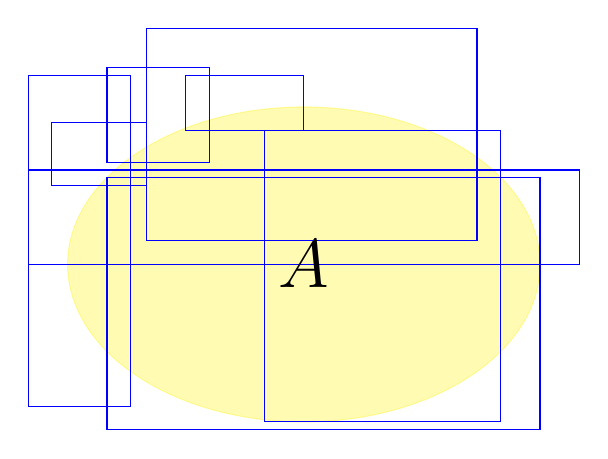
\begin{tikzpicture}
\draw[fill, yellow, opacity=0.3] (0,0) ellipse [x radius=3cm, y radius=2cm];
\draw[blue] (-3.2,1) rectangle (-2,1.8);
\draw[blue] (-2.5,1.3) rectangle (-1.2,2.5);
\draw[blue] (-1.5,1.7) rectangle (0,2.4);
\draw[blue] (-0.5,1.7) rectangle (2.5,-2);
\draw[blue] (-2.5,-2.1) rectangle (3,1.1);
\draw[blue] (-3.5,0) rectangle (3.5,1.2);
\draw[blue] (-3.5,-1.8) rectangle (-2.2,2.4);
\draw[blue] (-2,0.3) rectangle (2.2,3);
\node[] () at (0,0) {\Huge{\(A\)}};
\end{tikzpicture}
\end{center}
\emph{Two extreme cases:}
\begin{itemize}
\item If no such cover \(\{A_{i}\}_{i\in\N}\subseteq \mathcal{A}\) exists, then
\(\mu^*(A)=\infty\) \emph{(largest possible sum of premeasures)}.
\item If there is a cover \(\{A_{i}\}_{i\in\N}\subseteq \mathcal{A}\) of \(A\)
such that \(\mu_0(A_i)=0~\forall i\in\N\), then \(\mu^*(A)=0\) \emph{(smallest
possible sum of premeasures)}.
\end{itemize}
Now we show that \(\mu^*\) is an outer measure.
\begin{enumerate}[label={(\arabic*)}]
\item By setting \(A_i=\varnothing\in\mathcal{A}~\forall i\in\N\), we get a
cover of \(\varnothing\) such that \(\mu_0(A_i)=\mu_0(\varnothing)=0~\forall
i\in\N\), thus \(\mu^*(\varnothing)=0\).
\item Fix any \(A,B\subseteq \Omega\) with \(A\subseteq B\). Since every cover
\(\{A_{i}\}_{i\in\N}\subseteq \mathcal{A}\) of \(B\) must also cover \(A\) (but
not vice versa), we conclude that \(\mu^*(A)\le\mu^*(B)\) as we are
taking infimum over a larger number of covers for the former.
\item Fix any \(A_1,A_2,\dotsc\in\mathcal{P}(\Omega)\). In case
\(\mu^*(A_i)=\infty\) for some \(i\in\N\), the \(\sigma\)-subadditivity would
just be saying ``\(\infty\le\infty\)'', which trivially holds. Thus, assume
henceforth that \(\mu^*(A_i)<\infty\) for all \(i\in\N\).

Fix any \(i\in\N\). By definition of the infimum, for all \(\varepsilon>0\),
there exists a cover \(\{A_{ik}\}_{k\in\N}\) of \(A_i\) such that
\(\sum_{k=1}^{\infty}\mu_0(A_{ik})\le\mu^*(A_i)+\varepsilon/2^i\).  Collecting
these covers for all \(i\in\N\) together yields a cover of
\(\bigcup_{i=1}^{\infty}A_i\) since
\(\bigcup_{i=1}^{\infty}\bigcup_{k=1}^{\infty}A_{ik}\supseteq
\bigcup_{i=1}^{\infty}A_i\). Then consider:
\[
\mu^*\left(\bigcup_{i=1}^{\infty}A_i\right)
\overset{\text{(infimum)}}{\le}
\underbrace{\sum_{i=1}^{\infty}\sum_{k=1}^{\infty}\mu_0(A_{ik})}_{\mathclap{\text{sum
of premeasures for \emph{one} cover}}}
\le\sum_{i=1}^{\infty}(\mu^*(A_i)+\varepsilon/2^i)
=\varepsilon+\sum_{i=1}^{\infty}\mu^*(A_i)
\]
As this holds for all \(\varepsilon>0\), we conclude that
\(\mu^*(\bigcup_{i=1}^{\infty}A_i)\le\sum_{i=1}^{\infty}\mu^*(A_i)\).
\end{enumerate}

\subsection*{Goal: Showing that \(\mu^*\) extends \(\mu_0\).}
\emph{Idea:} We start with a \emph{semiring} \(\mathcal{A}\) on which \(\mu_0\)
is defined. To show the desired extension, we would need to first show the
monotonicity and \(\sigma\)-subadditivity of \(\mu_0\). However, the semiring
\(\mathcal{A}\) itself does not have enough ``structure'' for us to do that,
thus we need to use a somewhat indirect approach which considers a \emph{ring
\(\mathcal{A}_{\uplus}\) generated by \(\mathcal{A}\)}, and prove those two
properties on the ring \(\mathcal{A}_{\uplus}\supseteq \mathcal{A}\), which
would then imply the properties hold on \(\mathcal{A}\) as well.

\textbf{Showing that
\(\mathcal{A}_{\uplus}:=\{\biguplus_{i=1}^{n}A_i:A_i\in\mathcal{A}, n\in\N\}\)
is a ring \emph{(ring generated by \(\mathcal{A}\))}.} It is clear that
\(\mathcal{A}_{\uplus}\supseteq \mathcal{A}\) by considering one-set unions.

Note that \(\mathcal{A}_{\uplus}\) is a \(\pi\)-system since for all
\(A,B\in\mathcal{A}_{\uplus}\), we can write \(A=\bigcup_{i=1}^{n}A_i\) and
\(B=\biguplus_{j=1}^{m}B_j\), so \(A\cap
B=\bigcup_{i=1}^{n}\bigcup_{j=1}^{m}\underbrace{(A_i\cap
B_j)}_{\mathclap{\text{\(\in\mathcal{A}\) due to closedness under
intersections}}}\) is a finite disjoint union of sets in \(\mathcal{A}\), thus
\(A\cap B\in\mathcal{A}_{\uplus}\).

Now we show that \(\mathcal{A}_{\uplus}\) is a ring.
\begin{enumerate}[label={(\arabic*)}]
\item Since \(\varnothing\in\mathcal{A}\), we have
\(\varnothing\in\mathcal{A}_{\uplus}\) (take \(n=1\) and \(A_1=\varnothing\)).
\item Fix any \(A,B\in\mathcal{A}_{\uplus}\). Then write
\(A=\biguplus_{i=1}^{n}A_i\) and \(B=\biguplus_{j=1}^{m}B_j\). Hence,
\[
A\setminus B=\left(\biguplus_{i=1}^{n}A_i\right)\setminus \left(\biguplus_{j=1}^{m}B_j\right)
=\biguplus_{i=1}^{n}\left(\vc{A_i\setminus \left(\biguplus_{j=1}^{m}B_j\right)}\right)
\overset{\text{(\Cref{lma:diff-mult-sets})}}{=}
=\biguplus_{i=1}^{n}\vc{\biguplus_{k=1}^{p}\underbrace{C_{ik}}_{\in\mathcal{A}}},
\]
which is a finite disjoint union of sets in \(\mathcal{A}\), thus belongs to
\(\mathcal{A}_{\uplus}\).
\item Fix any \(A,B\in\mathcal{A}_{\uplus}\). Then from above we know
\(A\setminus B\in\mathcal{A}_{\uplus}\). Also, \(A\cap
B\in\mathcal{A}_{\uplus}\) as \(\mathcal{A}_{\uplus}\) is a \(\pi\)-system.
So both \(A\setminus B\) and \(A\cap B\) are finite disjoint unions of sets in
\(\mathcal{A}\), hence \(A\cup B=(A\setminus B)\uplus(A\cap B)\) is a finite
disjoint union of sets in \(\mathcal{A}\), which belongs to \(\mathcal{A}_{\uplus}\).
\end{enumerate}
\textbf{Extending \(\mu_0\) from \(\mathcal{A}\) to \(\mathcal{A}_{\uplus}\).}
To perform the extension, we define
\(\mu_0(\biguplus_{i=1}^{n}A_i):=\sum_{i=1}^{n}\mu_0(A_i)\) for all \(A_1,\dotsc,A_n\in\mathcal{A}\).
(By considering union of one set, we see that the measures assigned for sets in
\(\mathcal{A}\) remain unchanged, aligning with the extension property.) Now we
will show that such extended \(\mu_0\) is well-defined (which would then imply
uniqueness).

Suppose we have \(\biguplus_{i=1}^{n}A_i=\biguplus_{j=1}^{m}B_j\) where \(A_1,\dotsc,A_n,B_1,\dotsc,B_m\in\mathcal{A}\).
Then we have \(A_i\overset{(A_i\subseteq \biguplus_{i=1}^{n}A_i)}{=}
A_i\cap\biguplus_{i=1}^{n}A_i=A_i\cap\biguplus_{j=1}^{m}B_j=\biguplus_{j=1}^{m}(\vc{A_i\cap
B_j})\). Thus, by finite additivity of \(\mu_0\) on \(\mathcal{A}\), we have
\(\mu_0(A_i)=\sum_{j=1}^{m}\mu_0(\vc{A_i\cap B_j})\). Therefore,
\[
\sum_{i=1}^{n}\mgc{\mu_0(A_i)}=\sum_{i=1}^{n}\mgc{\sum_{j=1}^{m}\mu_0(A_i\cap B_j)}
=\sum_{j=1}^{m}\orc{\sum_{i=1}^{n}\mu_0(B_j\cap A_i)}
\overset{\text{(similar argument)}}{=}\sum_{j=1}^{m}\orc{\mu_0(B_j)},
\]
establishing the well-definedness.

\textbf{Showing that \(\mu_0\) is a premeasure on
\(\mathcal{A}_{\uplus}\).} As \(\mu_0\) is already a premeasure on
\(\mathcal{A}\), it suffices to show \(\sigma\)-additivity of \(\mu_0\) on
\(\mathcal{A}_{\uplus}\) (which is a ring, hence also a semiring).

Fix any pairwise disjoint \(A_1,A_2,\dotsc\in\mathcal{A}_{\uplus}\) \vc{with
\(\biguplus_{i=1}^{\infty}A_i\in\mathcal{A}_{\uplus}\)} (don't miss \warn{}).  Then, we
can express each \(A_i\) as a disjoint union of sets in \(\mathcal{A}\).
Symbolically, we can write \(\gc{A_i=\biguplus_{j=1}^{n_i}A_{ij}}~\forall i\in\N\).
As \(A_i\)'s are also pairwise disjoint themselves, we know the \(A_{ij}\)'s
(across both \(i\) and \(j\)) are pairwise disjoint.

Note that we can write \(\biguplus_{i=1}^{\infty}\gc{A_i}
=\biguplus_{i=1}^{\infty}\gc{\biguplus_{j=1}^{n_i}A_{ij}}\), which is a
countable disjoint union of sets in \(\mathcal{A}\) (those \(A_{ij}\)'s).
Hence, we have
\[
\mu_0\left(\biguplus_{i=1}^{\infty}A_i\right)
\overset{\text{(\(\sigma\)-add.~on \(\mathcal{A}\))}}{=}\sum_{i=1}^{\infty}\orc{\sum_{j=1}^{n_i}\mu_0(A_{ij})}
\overset{\text{(extension of \(\mu_0\))}}{=}\sum_{i=1}^{\infty}\orc{\mu_0\left(\biguplus_{j=1}^{n_i}A_{ij}\right)}
=\sum_{i=1}^{\infty}\mu_0(A_i).
\]
\textbf{Showing the monotonicity and \(\sigma\)-subadditivity of \(\mu_0\) on
\(\mathcal{A}_{\uplus}\).} Techniques similar to the ones used for proving the
monotonicity and \(\sigma\)-subadditivity of a general measure in
\labelcref{it:meas-prop} can be utilized here.
\begin{itemize}
\item \emph{Monotonicity:}
Fix any \(A,B\in\mathcal{A}_{\uplus}\) with \(A\subseteq B\).  Note that
\(\vc{A=A\cap B}\overset{\text{(ring \(\Rightarrow\)
semiring)}}{\in}\mathcal{A}_{\uplus}\), and \(B\setminus
A\in\mathcal{A}_{\uplus}\) by closedness under set differences.  Hence, writing
\(B=(A\cap B)\uplus (B\setminus A)\in\mathcal{A}_{\uplus}\) gives
\[
\mu(B)\overset{\text{(finite additivity)}}{=}\vc{\mu(A\cap B)}+\mu(B\setminus A)
=\vc{\mu(A)}+\underbrace{\mu(B\setminus A)}_{\ge 0}
\ge \mu(A).
\]
\item \emph{\(\sigma\)-subadditivity:} Fix any
\(A_1,A_2,\dotsc\in\mathcal{A}_{\uplus}\) with \(\bigcup_{i=1}^{\infty}A_i
\in\mathcal{A}_{\uplus}\).  Let \(B_1:=A_1\in\mathcal{A}_{\uplus}\) and
\(B_n:=A_n\setminus \bigcup_{i=1}^{n-1}A_i\in\mathcal{A}_{\uplus}\) for every
integer \(n\ge 2\).  Then by construction, (i) \(B_n\)'s are disjoint, (ii)
\(B_n\subseteq A_n\) for every \(n\in\N\), and (iii)
\(\bigcup_{i=1}^{n}A_i=\biguplus_{i=1}^{n}B_i\) for every \(n\in\N\).

By (iii), we have \(\bigcup_{i=1}^{\infty}A_i
=\lim_{N\to\infty}\bigcup_{i=1}^{N}A_i =\lim_{N\to\infty}\biguplus_{i=1}^{N}B_i
=\biguplus_{i=1}^{\infty}B_i \). Thus,
\[
\mu\left(\bigcup_{i=1}^{\infty}A_i\right)
=\mu\left(\biguplus_{i=1}^{\infty}B_i\right)
=\sum_{i=1}^{\infty}\mu(B_i)
\overset{\text{(ii), monotonicity}}{\le}\sum_{i=1}^{\infty}\mu(A_i).
\]
\end{itemize}
\textbf{Showing that \(\mu^*\) extends \(\mu_0\) on \(\mathcal{A}\).} Fix any
\(A\in\mathcal{A}\) and any cover \(\{A_{i}\}_{i\in\N}\subseteq \mathcal{A}\)
of \(A\). Then, we have \(\bigcup_{i=1}^{\infty}A_i\supseteq A\), which implies
\(\vc{\bigcup_{i=1}^{\infty}(A_i\cap A)}=\left(\bigcup_{i=1}^{\infty}A_i\right)\cap A=\vc{A}\). Thus,
\begin{align*}
\mu_0(A)&=\mu_0\left(\vc{\bigcup_{i=1}^{\infty}(A_i\cap A)}\right)
\overset{\text{(\(\sigma\)-subadditivity)}}{\le}
\sum_{i=1}^{\infty}\mu_0(A_i\cap A)
=\lim_{n\to\infty}\sum_{i=1}^{n}\mu_0(A_i\cap A) \\
&\overset{\text{(monotonicity, \(A_i\cap A\subseteq A\))}}{\le}
\lim_{n\to\infty}\sum_{i=1}^{n}\mu_0(A_i)
=\mgc{\sum_{i=1}^{\infty}\mu_0(A_i)}.
\end{align*}
As this holds for all covers \(\{A_{i}\}_{i\in\N}\subseteq \mathcal{A}\) of
\(A\), \(\mu_0(A)\) is a lower bound for the \mgc{sums of premeasures} of the covers.
Since the infimum is the greatest lower bound, we have
\(\mu_0(A)\le\mu^*(A)\).

On the other hand, note that \(\{A,\varnothing,\varnothing,\dotsc\}\subseteq
\mathcal{A}\) is a cover of \(A\), and \(\mu_0(A)\) is the sum of premeasures
for this cover. So, \(\mu^*(A)\overset{\text{(infimum)}}{\le}\mu_0(A)\). Hence
we have \(\mu^*(A)=\mu_0(A)~\forall A\in\mathcal{A}\), meaning that \(\mu^*\)
extends \(\mu_0\) on \(\mathcal{A}\).

\subsection*{Goal: Applying the principle of good sets to show that every set in
\(\sigma(\mathcal{A})\) is Carath\'edory-measurable}
Let \(\mathcal{A^*}:=\{A\subseteq \Omega:\mu^*(B)=\mu^*(B\cap A)+\mu^*(B\cap
A^c)~\forall B\subseteq \Omega\}\) be the family of all
\defn{Carath\'eodory-measurable sets}, or ``good'' sets. To apply the principle
of good sets, we will show that (i) \(\mathcal{A}\subseteq \mathcal{A}^*\) and
(ii) \(\mathcal{A}^*\) is a \(\sigma\)-algebra, which would then imply that
every set in \(\sigma(\mathcal{A})\) is ``good'' (Carath\'edory-measurable).

\textbf{Showing that \(\mathcal{A}\subseteq \mathcal{A}^*\).}
Fix any \(A\in\mathcal{A}\) and any \(B\subseteq \Omega\). Using a property of
the infimum, for all \(\varepsilon>0\), there is a cover
\(\{A_{i}\}_{i\in\N}\subseteq \mathcal{A}\) of \(B\) such that
\(\sum_{i=1}^{\infty}\mu_0(A_i)\le\mgc{\mu^*(B)+\varepsilon}\).
Let \(E_i:=A_i\cap A\overset{\text{(semiring)}}{\in}\mathcal{A}\) for every \(i\in\N\).
Then, for every \(i\in\N\), we have \(A_i\setminus A=\vc{A_i\setminus
E_i\overset{\text{(semiring)}}{=}\biguplus_{j=1}^{n_i}B_{ij}}\) for some pairwise
disjoint \(B_{i1},\dotsc,B_{in_i}\in\mathcal{A}\).

Thus, we have:
\begin{itemize}
\item \(A_i=E_i\uplus\vc{(A_i\setminus E_i)}=E_i\uplus\vc{\bigcup_{j=1}^{n_i}B_{ij}}\).
\item \(B\cap A\overset{\text{(cover)}}{\subseteq}
\left(\bigcup_{i=1}^{\infty}A_i\right)\cap A
=\bigcup_{i=1}^{\infty}(A_i\cap A)
=\orc{\bigcup_{i=1}^{\infty}E_i}\).
\item \(B\setminus A\overset{\text{(cover)}}{\subseteq}
\left(\bigcup_{i=1}^{\infty}A_i\right)\setminus A
=\bigcup_{i=1}^{\infty}(A_i\setminus A)
=\bigcup_{i=1}^{\infty}\vc{\biguplus_{j=1}^{n_i}B_{ij}}.
\)
\end{itemize}
Hence,
\begin{align*}
\mu^*(B\cap A)+\mu^*(B\setminus A)
&\overset{\text{(monotonicity)}}{\le}
\mu^*\left(\orc{\bigcup_{i=1}^{\infty}E_i}\right)
+\mu^*\left(\bigcup_{i=1}^{\infty}\vc{\biguplus_{j=1}^{n_i}B_{ij}}\right) \\
&\overset{\text{(\(\sigma\)-subadditivity)}}{\le}
\sum_{i=1}^{\infty}\mu^*(E_i)+\sum_{i=1}^{\infty}\sum_{j=1}^{n_i}\mu^*(B_{ij}) \\
&\overset{\text{(\(\mu^*\) extends \(\mu\) on \(\mathcal{A}\))}}{=}\sum_{i=1}^{\infty}\mu_0(E_i)+\sum_{i=1}^{\infty}\sum_{j=1}^{n_i}\mu_0(B_{ij}) \\
&=\sum_{i=1}^{\infty}\left(\mu_0(E_i)+\sum_{j=1}^{n_i}\mu_0(B_{ij})\right)
=\sum_{i=1}^{\infty}\mu\left(E_i\uplus\vc{\bigcup_{j=1}^{n_i}B_{ij}}\right)
=\sum_{i=1}^{\infty}\mu_0(A_i)
\le\mgc{\mu^*(B)+\varepsilon}
\end{align*}
for all \(\varepsilon>0\), which implies \(\mu^*(B\cap A)+\mu^*(B\setminus A)
\le\mu^*(B)\). On the other hand, by finite subadditivity we have
\(\mu^*(B)\le\mu^*(B\cap A)+\mu^*(B\setminus A)\). So \(\mu^*(B)=\mu^*(B\cap
A)+\mu^*(B\setminus A)\). As this holds for all \(B\subseteq \Omega\), we have
\(A\in\mathcal{A}^*\). This shows \(\mathcal{A}\subseteq \mathcal{A}^*\).

\textbf{Showing that \(\mathcal{A}^*\) is a \(\sigma\)-algebra on
\(\Omega\).} Due to \Cref{prp:dynkin-prop}, we will show that
\(\mathcal{A}^*\) is a \(\sigma\)-algebra on \(\Omega\) by showing it is
both (i) \(\pi\)-system and (ii) Dynkin system.

\begin{itemize}
\item \emph{\(\pi\)-system:}
\begin{enumerate}[label={(\arabic*)}]
\item For all \(B\subseteq \Omega\), we have
\(\mu^*(B\cap\varnothing)+\mu^*(B\cap\varnothing^c)
=\mu^*(\varnothing)+\mu^*(B\cap\Omega)=\mu^*(B)\). Thus
\(\varnothing\in\mathcal{A}^*\). This shows the nonemptyness.
\item Fix any \(A_1,A_2\in\mathcal{A}^*\) and any \(B\subseteq \Omega\).
Observe that \((\vc{A_1\cap A_2})^c
=\mgc{(A_1^c\cap A_2)}\uplus \blc{(A_1\cap A_2^c)}\uplus \orc{(A_1^c\cap A_2^c)}
\).
\begin{center}
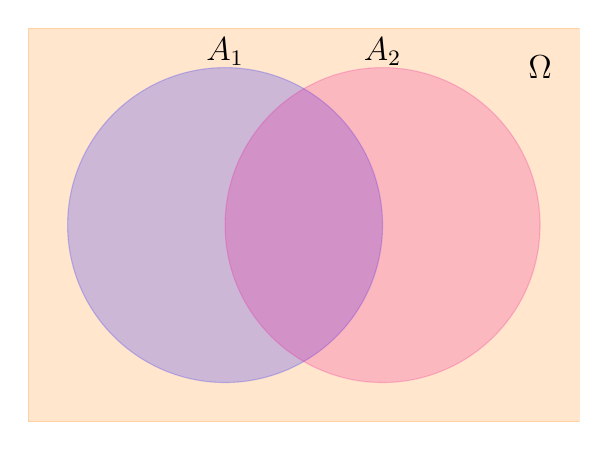
\begin{tikzpicture}
\draw[fill, orange, opacity=0.2] (-2.5,-2.5) rectangle (4.5,2.5);
\draw[fill, blue, opacity=0.2] (0,0) circle [radius=2cm];
\draw[fill, magenta, opacity=0.2] (2,0) circle [radius=2cm];
\node[] () at (0,2.2) {\large{\(A_1\)}};
\node[] () at (2,2.2) {\large{\(A_2\)}};
\node[] () at (4,2) {\large{\(\Omega\)}};
\end{tikzpicture}
\end{center}
Hence, we have
\begin{align*}
&\mu^*(B\cap\gc{(A_1\cap A_2)})+\mu^*(B\cap\gc{(A_1\cap A_2)^{c}}) \\
&\quad=\mu^*(B\cap A_1\cap A_2)
+\mu^*(B\cap(\mgc{(A_1^c\cap A_2)}\uplus \blc{(A_1\cap A_2^c)}\uplus \orc{(A_1^c\cap A_2^c)})) \\
&\quad\overset{\text{(finite subadditivity)}}{\le}
\mu^*(B\cap A_1\cap A_2)
+\mu^*(B\cap\mgc{A_1^c\cap A_2})
+\mu^*(B\cap\blc{A_1\cap A_2^c})
+\mu^*(B\cap\orc{A_1^c\cap A_2^c}) \\
&\quad=\mu^*(\vc{B\cap A_2}\cap A_1)
+\mu^*(\vc{B\cap A_2}\cap A_1^c)
+\mu^*(\brc{B\cap A_2^c}\cap A_1)
+\mu^*(\brc{B\cap A_2^c}\cap A_1^c) \\
&\quad\underset{(B\cap A_2,\; B\cap A_2^c\subseteq \Omega)}{\overset{(A_1\in\mathcal{A}^*)}{=}}
\mu^*(\vc{B\cap A_2})+\mu^*(\brc{B\cap A_2^c})
=\mu^*(B).
\end{align*}
On the other hand, by finite subadditivity we have
\(\mu^*(B\cap\gc{(A_1\cap A_2)})+\mu^*(B\cap\gc{(A_1\cap A_2)^{c}})\ge
\mu(B)\).
So the equality holds and \(A_1\cap A_2\in\mathcal{A}^*\).
\end{enumerate}
\item \emph{Dynkin system:}
\begin{enumerate}[label={(\arabic*)}]
\item We have shown that \(\varnothing\in\mathcal{A}^*\) above.
\item From the definition of \(\mathcal{A}^*\), we can clearly see that
\(A\in\mathcal{A}^*\) iff \(A^c\in\mathcal{A}^*\).
\item Fix any pairwise disjoint \(A_1,A_2,\dotsc\in\mathcal{A}^*\). Let
\(\widetilde{A}_n:=\biguplus_{i=1}^{n}A_i\) for every \(n\in\N\) and
\(\widetilde{A}_{\infty}:=\biguplus_{i=1}^{\infty}A_i\). By De Morgan's law, we
have \(\widetilde{A}_n=(\bigcap_{i=1}^{n}A_i^c)^{c}\in\mathcal{A}^*\), since
\(\mathcal{A}^*\) is closed under complements (proven above) and intersections
(as it is shown to be a \(\pi\)-system).

Now, note that for all \(B\subseteq \Omega\), we have \(\forall n\in\N\),
\[
\blc{\mu^*(B\cap\widetilde{A}_{n+1})}
\overset{(\widetilde{A}_{n}\in\mathcal{A}^*)}{=}
\mu^*((B\cap\widetilde{A}_{n+1})\cap \vc{\widetilde{A}_{n}})
+\mu^*((B\cap\widetilde{A}_{n+1})\cap \vc{(\widetilde{A}_{n})^c})
=\blc{\mu^*(B\cap\widetilde{A}_n)}+\mu^*(B\cap A_{n+1})
\]
Noting that \(\widetilde{A}_{1}=A_1\), this recursive relationship yields
\(\mu^*(B\cap\widetilde{A}_{n})=\sum_{i=1}^{n}\mu^*(B\cap A_i)~\forall
n\in\N\).

Then consider, for all \(n\in\N\),
\begin{align*}
\mu^*((B\cap\widetilde{A}_{\infty})\cup(B\cap\widetilde{A}_{\infty}^{c}))
&=\mu^*(B)
\overset{(\widetilde{A}_{n}\in\mathcal{A}^*)}{=}
\mu^*(B\cap\widetilde{A}_n)+\mgc{\mu^*(B\cap\widetilde{A}_n^{c})} \\
&\overset{\text{(monotonicity)}}{\ge}
\orc{\mu^*(B\cap\widetilde{A}_n)}+\mgc{\mu^*(B\cap\widetilde{A}_{\infty}^{c})} \\
&=\orc{\sum_{i=1}^{n}\mu^*(B\cap A_i)}+\mu^*(B\cap\widetilde{A}_{\infty}^{c}).
\end{align*}
As this holds for all \(n\in\N\), taking limit \(n\to\infty\) gives
\begin{align}
\label{eq:mu-star-geq-sum}\mu^*((B\cap\widetilde{A}_{\infty})\cup(B\cap\widetilde{A}_{\infty}^{c}))
&\ge\orc{\sum_{i=1}^{\infty}\mu^*(B\cap A_i)}+\mu^*(B\cap\widetilde{A}_{\infty}^{c}) \\
\nonumber&\overset{\text{(\(\sigma\)-subadditivity)}}{\ge}
\mu^*\left(\biguplus_{i=1}^{\infty}(B\cap A_i)\right)+\mu^*(B\cap\widetilde{A}_{\infty}^{c}) \\
\nonumber&\overset{\text{(distributivity)}}{=}\mu^*(B\cap\widetilde{A}_{\infty})+\mu^*(B\cap\widetilde{A}_{\infty}^{c}).
\end{align}
On the other hand, by finite subadditivity we have
\[
\mu^*((B\cap\widetilde{A}_{\infty})\cup(B\cap\widetilde{A}_{\infty}^{c}))
\le\mu^*(B\cap\widetilde{A}_{\infty})+\mu^*(B\cap\widetilde{A}_{\infty}^{c}).
\]
Hence the equality holds and \(\widetilde{A}_{\infty}\in\mathcal{A}^*\).
\end{enumerate}
\end{itemize}
\subsection*{Goal: Extending uniquely \(\mu_0\) to a \(\sigma\)-finite measure \(\mu\)
on \(\sigma(\mathcal{A})\)}
\textbf{Showing that \(\mu^*\) is a measure on the \(\sigma\)-algebra \(\mathcal{A}^*\).}
\begin{enumerate}[label={(\arabic*)}]
\item We can view the outer measure \(\mu^*\) as a function on
\(\mathcal{A}^*\subseteq \mathcal{P}(\Omega)\). Also its codomain is
\([0,\infty]\) by the definition of outer measure.
\item By the definition of outer measure, we have \(\mu^*(\varnothing)=0\).
\item Setting \(B=\widetilde{A}_{\infty}\) in \labelcref{eq:mu-star-geq-sum} gives
\(\mu^*(\widetilde{A}_{\infty})\ge\sum_{i=1}^{\infty}\mu^*(A_i)\). On the other
hand, by \(\sigma\)-subadditivity we have
\(\mu^*(\widetilde{A}_{\infty})\le\sum_{i=1}^{\infty}\mu^*(A_i)\). Thus the
equality holds, implying the \(\sigma\)-additivity on \(\mathcal{A}^*\).
\end{enumerate}

\textbf{Extending \(\mu_0\) to a measure \(\mu\).} By the principle of good
sets, we have previously shown that \(\sigma(\mathcal{A})\subseteq
\mathcal{A}^*\). Thus we can define the restriction
\(\mu:=\mu^*|_{\sigma(\mathcal{A})}\), which is a measure on
\(\sigma(\mathcal{A})\). (The underlying measure space is
\((\Omega,\sigma(\mathcal{A}),\mu)\).) Also, note that
\(\mu|_{\mathcal{A}}\overset{(\mathcal{A}\subseteq \sigma(\mathcal{A}))}{=}
\mu^*|_{\mathcal{A}}\overset{\text{(\(\mu^*\) extends
\(\mu_0\))}}{=}\mu_0|_{\mathcal{A}}\), so \(\mu\) extends \(\mu_0\).

\textbf{Showing the \(\sigma\)-finiteness of \(\mu\) and the uniqueness of such measure.}
\begin{itemize}
\item \emph{\(\sigma\)-finiteness:}
By assumption, \(\mu_0\) is \(\sigma\)-finite on \(\mathcal{A}\), i.e.,
\(\Omega=\bigcup_{i=1}^{\infty}A_i\) for some \(A_1,A_2,\dotsc\in\mathcal{A}\subseteq\sigma(\mathcal{A})\)
with \(\mu_0(A_i)<\infty~\forall i\in\N\). Since
\(\mu|_{\mathcal{A}}=\mu_0|_{\mathcal{A}}\), we have also
\(\mu(A_i)<\infty~\forall i\in\N\), thus \(\mu\) is \(\sigma\)-finite.
\item \emph{Uniqueness:} Note that the semiring \(\mathcal{A}\) is also a
\(\pi\)-system, and that the \emph{\(\sigma\)-finiteness on
\(\mathcal{A}\)} is satisfied. Thus, by \Cref{prp:meas-unique}, another
\(\sigma\)-finite measure \(\nu\) on \(\sigma(\mathcal{A})\) that extends
\(\mu_0\) must coincide with \(\mu\), establishing the uniqueness.
\end{itemize}
\end{pf}

\item \label{it:meas-complete-wlog} By \Cref{thm:complete-meas}, a measure can
always be made complete, including the extension \(\mu\) here. Hence, by
replacing it with the completed version if necessary, we may assume that the
measure \(\mu\) extended from \(\mu_0\) in \Cref{thm:caratheodory} is complete;
this will be assumed henceforth.
\end{enumerate}
\subsection{Borel Measures on \(\R^d\)}
\label{subsect:borel-meas-rd}
\begin{enumerate}
\item One main application of \Cref{thm:caratheodory} is to construct
\emph{Borel measures} on \(\R^d\), which include the frequently used
\emph{Lebesgue measure} on \(\R^d\) (corresponding to our usual notion of
``volume'') as a special case.

\item \textbf{Preliminary concepts.} Let us first go through some concepts to
be used in the construction. A function \(F:\R^d\to\R\) is:
\begin{itemize}
\item \defn{right-continuous} if \(F(\vect{x})=\lim_{\vect{h}\to
\vect{0}^{+}}F(\vect{x}+\vect{h})=:F(\vect{x}+)\) for all \(\vect{x}\in\R^d\).
\item \defn{grounded} if \(\lim_{x_j\to -\infty}F(\vect{x})=0\) (with
\(\vect{x}=(x_1,\dotsc,x_n)\)) for all \(j=1,\dotsc,d\)
\item \defn{\(d\)-increasing} if \(\Delta_{(\vect{a},\vect{b}]}F\ge 0\) for all
\(\vect{a}\le\vect{b}\), where \(\Delta_{(\vect{a},\vect{b}]}F\) is the
\defn{\(F\)-volume} (over \((\vect{a},\vect{b}]\)):
\begin{align*}
\Delta_{(\vect{a},\vect{b}]}F&:=
\sum_{\vect{i}\in\{0,1\}^{d}}^{}(-1)^{i_{1}+\dotsb+i_{d}}
F\left(a_1^{i_1}b_1^{1-i_1},\dotsc,a_{d}^{i_d}b_{d}^{1-i_{d}}\right) \\
&\overset{\text{(in words)}}{=}
\sum_{\vect{i}\in\{0,1\}^{d}}^{}
(\text{alternating \(+\)/\(-\) sign})\;
F\left(
\begin{cases}
b_1&\text{if \(i_1=0\)} \\
a_1&\text{if \(i_1=1\)}
\end{cases}
,\dotsc,
\begin{cases}
b_d&\text{if \(i_d=0\)} \\
a_d&\text{if \(i_d=1\)}
\end{cases}
\right),
\end{align*}
with \(\vect{i}=(i_1,\dotsc,i_d)\), \(\vect{a}=(a_1,\dotsc,a_d)\), and
\(\vect{b}=(b_1,\dotsc,b_d)\).

Examples:
\begin{itemize}
\item \emph{(\(d=1\))} \(\Delta_{(a_1,b_1]}F=F(b_1)-F(a_1)\).
\begin{note}
In this case, \emph{\(d\)-increasing} coincides with our usual notion of \emph{increasing}.
\end{note}
\item \emph{(\(d=2\))} \(\Delta_{(a_1,b_1]\times (a_2,b_2]}F
=F(b_1,b_2)-F(a_1,b_2)-F(b_1,a_2)+F(a_1,a_2)\).

Note that:
\begin{itemize}
\item \(\mgc{\Delta_{(a_2,b_2]}^{(2)}}\gc{\Delta_{(a_1,b_1]}^{(1)}}F(x_1,x_2)
=\gc{\Delta_{(a_1,b_1]}^{(1)}}F(x_1,\mgc{b_2})-\gc{\Delta_{(a_1,b_1]}^{(1)}}F(x_1,\mgc{a_2})
=F(\gc{b_1},\mgc{b_2})-F(\gc{a_1},\mgc{b_2})
-(F(\gc{b_1},\mgc{a_2})-F(\gc{a_1},\mgc{a_2}))
=\Delta_{(a_1,b_1]\times (a_2,b_2]}F\).
\item \(\gc{\Delta_{(a_1,b_1]}^{(1)}}\mgc{\Delta_{(a_2,b_2]}^{(2)}}F(x_1,x_2)
=\mgc{\Delta_{(a_2,b_2]}^{(2)}}F(\gc{b_1},x_2)-\mgc{\Delta_{(a_2,b_2]}^{(2)}}F(\gc{a_1},x_2)
=F(\gc{b_1},\mgc{b_2})-F(\gc{b_1},\mgc{a_2})
-(F(\gc{a_1},\mgc{b_2})-F(\gc{a_1},\mgc{a_2}))
=\Delta_{(a_1,b_1]\times (a_2,b_2]}F\).
\end{itemize}
\begin{note}
The notation \(\Delta_{(a,b]}^{(i)}F(x_1,\dotsc,x_n)\) refers to the
\emph{first-order difference} with \(i\)th input of \(F\) substituted, i.e.,
\(F(x_1,\dotsc,x_{i-1},b,x_{i+1},\dotsc,x_n)-F(x_1,\dotsc,x_{i-1},a,x_{i+1},\dotsc,x_n)\).
Note that the \(i\)th input in the parenthesis would not affect the first-order
difference (as it will get substituted anyway), but the other inputs matter as
they would remain the same in the resulting expressions. For convenience in
notations, sometimes we will drop the superscript ``\((i)\)'' when the meaning
is clear from context.
\end{note}
\end{itemize}
\end{itemize}

Before proceeding further, let us also introduce some special notations that
will be useful later on. Let \(J\subseteq \{1,\dotsc,d\}\). Then we have the
following notations for vectors:
\begin{itemize}
\item \(\vect{x}_{J}:=(x_{j})_{j\in J}\).
\item \(\vect{x}_{J^c}:=(x_j)_{j\notin J}\).
\item For all \(x\in\R\), \({}_{d}x:=(x,\dotsc,x)\in\R^d\).
\item For all \(\vect{x}=(x_1,\dotsc,x_d),\vect{y}=(y_1,\dotsc,y_d)\in\R^d\):
\begin{itemize}
\item \(\vect{x}_{J\leftarrow\vect{y}_{J}}:=
\begin{cases}
x_j&\text{if \(j\notin J\),} \\
y_j&\text{if \(j\in J\)}.
\end{cases}
\)
\item \emph{Special case:} If \(J=\{j\}\), we may simply write
\(\vect{x}_{j\leftarrow y_j}\) instead of
\(\vect{x}_{J\leftarrow\vect{y}_{J}}\). More explicitly, we can write
\(\vect{x}_{j\leftarrow y_j}=(x_1,\dotsc,x_{j-1},y_j,x_{j+1},\dotsc,x_d)\).
\end{itemize}
\end{itemize}
\item\label{it:f-vol-prop} \textbf{Properties of \(F\)-volumes.} The definition of the \(F\)-volume
above may not be intuitive. So to understand it better, we will study some of
its properties. Let \(F:\R^d\to\R\) be a function.
\begin{enumerate}
\item\label{it:f-vol-permut} \emph{(permutation of first-order differences)} We
have \(\Delta_{(\vect{a},\vect{b}]}F
=\Delta_{(a_d,b_d]}\dotsb\Delta_{(a_1,b_1]}F(x_1,\dotsc,x_d)\) (or just
\(\Delta_{(a_d,b_d]}\dotsb\Delta_{(a_1,b_1]}F\)), and the order of
``\(\Delta\)''s can be freely changed.
\item\label{it:f-vol-mono} \emph{(monotonicity)} If \(F\) is \(d\)-increasing, then
\((\vect{a},\vect{b}]\subseteq (\vect{\alpha},\vect{\beta}]\implies \Delta_{(\vect{a},\vect{b}]}F
\le\Delta_{(\vect{\alpha},\vect{\beta}]}F\).
\item\label{it:f-vol-prod-diff} \emph{(product of differences)} If \(F(\vect{x})=\prod_{j=1}^{d}F_j(x_j)\), then
\(\Delta_{(\vect{a},\vect{b}]}F=\prod_{j=1}^{d}(F_{j}(b_j)-F_{j}(a_j))\).
\item\label{it:ground-lim} If \(F\) is grounded, then
\(\lim_{\vect{a}\to\vect{-\infty}}\Delta_{(\vect{a},\vect{x}]}F=:\Delta_{(\vect{-\infty},\vect{x}]}F=F(\vect{x})\)
for all \(\vect{x}\in\R^d\).
\item\label{it:f-vol-nonneg} \emph{(nonnegativity)} If \(F\) is grounded and \(d\)-increasing, and
\(J\) is strictly between \(\varnothing\) and \(\{1,\dotsc,d\}\) (i.e,
\(\varnothing\subsetneq J\subsetneq \{1,\dotsc,d\}\)), then
\(\Delta_{(\vect{a}_{J},\vect{b}_{J}]}F(\vect{x})\ge 0\) for all
\(\vect{x}_{J^c}\in\R^{|J^c|}\).
\begin{note}
Particularly, by setting \(J=\{j\}\) for each \(j=1,\dotsc,d\), this result
suggests that \(F\) is componentwise increasing under such conditions.
\end{note}
\end{enumerate}
\begin{pf}
\begin{enumerate}
\item The possibility of freely reordering the first-order differences follows
from the commutativity of addition (see the \(d=2\) example above for an
illustration). So henceforth we will just prove \(\Delta_{(\vect{a},\vect{b}]}F
=\Delta_{(a_d,b_d]}\dotsb\Delta_{(a_1,b_1]}F\) for all \(d\in\N\).

The case \(d=1\) holds trivially as both sides are referring to the same
thing. Now assume for induction that the case \(d=k\) holds for a \(k\in\N\).
Then,
\begin{align*}
\Delta_{(\vect{a},\vect{b}]}F&=
\sum_{\vect{i}\in\{0,1\}^{d}}^{}(-1)^{i_{1}+\dotsb+i_{d}}
F(a_1^{i_1}b_1^{1-i_1},\dotsc,a_{d}^{i_d}b_{d}^{1-i_{d}}) \\
&=
\sum_{\vect{i}\in\{0,1\}^{d}: \vc{i_d=0}}^{}(-1)^{i_{1}+\dotsb+i_{d}}
F(a_1^{i_1}b_1^{1-i_1},\dotsc,a_{d-1}^{i_{d-1}}b_{d-1}^{1-i_{d-1}},\vc{b_d}) \\
&\quad-\sum_{\vect{i}\in\{0,1\}^{d}: \orc{i_d=1}}^{}(-1)^{i_{1}+\dotsb+i_{d}}
F(a_1^{i_1}b_1^{1-i_1},\dotsc,a_{d-1}^{i_{d-1}}b_{d-1}^{1-i_{d-1}},\orc{a_d}) \\
&=
\Delta_{(a_{d-1},b_{d-1}]}\dotsb\Delta_{(a_1,b_1]}F(x_1,\dotsc,x_{d-1},\mgc{b_d}) \\
&\quad-\Delta_{(a_{d-1},b_{d-1}]}\dotsb\Delta_{(a_1,b_1]}F(x_1,\dotsc,x_{d-1},\mgc{a_d})
\quad\text{(inductive hypothesis)} \\
&=\mgc{\Delta_{(a_d,b_d]}}\Delta_{(a_{d-1},b_{d-1}]}\dotsb\Delta_{(a_1,b_1]}F(x_1,\dotsc,x_d),
\end{align*}
so the case \(d=k+1\) holds, completing the proof by induction.
\item For all \(j=1,\dotsc,d\) with \(a_j\le b_j\), we have
\[\gc{\Delta_{(a_j,b_j]}}
\vc{\Delta_{(\vect{a}_{\{j\}^{c}},\vect{b}_{\{j\}^{c}}]}F(x_1,\dotsc,x_j,\dotsc,x_d)}
\overset{\text{\labelcref{it:f-vol-permut}}}{=}
\Delta_{(\vect{a},\vect{b}]}F\overset{\text{(\(d\)-increasing)}}{\ge}0,
\]
which implies that
\[
\vc{\Delta_{(\vect{a}_{\{j\}^{c}},\vect{b}_{\{j\}^{c}}]}F(x_1,\dotsc,\gc{b_j},\dotsc,x_d)}
-\vc{\Delta_{(\vect{a}_{\{j\}^{c}},\vect{b}_{\{j\}^{c}}]}F(x_1,\dotsc,\gc{a_j},\dotsc,x_d)}
\ge 0
\]
for all \(a_j\le b_j\). Thus, the function
\(x_j\mapsto\vc{\Delta_{(\vect{a}_{\{j\}^{c}},\vect{b}_{\{j\}^{c}}]}F(x_1,\dotsc,x_j,\dotsc,x_d)}\) is
increasing for every \(j=1,\dotsc,d\). Particularly, we have
\begin{align*}
&\vc{\Delta_{(\vect{a}_{\{j\}^{c}},\vect{b}_{\{j\}^{c}}]}F(x_1,\dotsc,\gc{\beta_j},\dotsc,x_d)}
-\vc{\Delta_{(\vect{a}_{\{j\}^{c}},\vect{b}_{\{j\}^{c}}]}F(x_1,\dotsc,\gc{\alpha_j},\dotsc,x_d)} \\
&\quad\ge
\vc{\Delta_{(\vect{a}_{\{j\}^{c}},\vect{b}_{\{j\}^{c}}]}F(x_1,\dotsc,\gc{b_j},\dotsc,x_d)}
-\vc{\Delta_{(\vect{a}_{\{j\}^{c}},\vect{b}_{\{j\}^{c}}]}F(x_1,\dotsc,\gc{a_j},\dotsc,x_d)}
\end{align*}
if \(\alpha_j\le a_j\le b_j\le\beta_j\), for every \(j=1,\dotsc,d\). Now, since
\((\vect{a},\vect{b}]\subseteq (\vect{\alpha},\vect{\beta}]\), applying this
iteratively gives \begin{align*}
\Delta_{(\vect{a},\vect{b}]}F
&\overset{\text{\labelcref{it:f-vol-permut}}}{=}
\Delta_{\orc{(a_d,b_d]}}\dotsb\Delta_{(a_1,b_1]}F
\le\Delta_{\orc{(\alpha_d,\beta_d]}}\Delta_{(a_{d-1},b_d]}\dotsb\Delta_{(a_1,b_1]}F \\
&\overset{\text{\labelcref{it:f-vol-permut}}}{=}
\Delta_{\mgc{(a_{d-1},b_d]}}\Delta_{\orc{(\alpha_d,\beta_d]}}\dotsb\Delta_{(a_1,b_1]}F
\le\Delta_{\mgc{(\alpha_{d-1},\beta_d]}}\Delta_{\orc{(\alpha_d,\beta_d]}}\dotsb\Delta_{(a_1,b_1]}F \\
&\le\dotsb\le\Delta_{(\vect{\alpha},\vect{\beta}]}F.
\end{align*}
\item We use an iterative argument:
\begin{align*}
\Delta_{(\vect{a},\vect{b}]}F&\overset{\text{\labelcref{it:f-vol-permut}}}{=}
\Delta_{(a_d,b_d]}\dotsb\Delta_{(a_2,b_2]}\Delta_{(a_1,b_1]}F(x_1,\dotsc,x_d) \\
&=\Delta_{(a_d,b_d]}\dotsb\Delta_{(a_2,b_2]}\vc{\Delta_{(a_1,b_1]}F(x_1)F(x_2)\dotsb F(x_d)} \\
&=\Delta_{(a_d,b_d]}\dotsb\Delta_{(a_2,b_2]}\vc{(F_1(b_1)-F_1(a_1))F(x_2)\dotsb F(x_d)} \\
&=\vc{(F_1(b_1)-F_1(a_1))}\Delta_{(a_d,b_d]}\dotsb\Delta_{(a_2,b_2]}F(x_2)\dotsb F(x_d) \\
&=\dotsb=\prod_{j=1}^{d}(F_j(b_j)-F_j(a_j)).
\end{align*}
\item For all \(\vect{x}\in\R^d\), we have
\begin{align}
\nonumber\Delta_{(\vect{-\infty},\vect{x}]}F
&=\lim_{\vect{a}\to\vect{-\infty}}\Delta_{(\vect{a},\vect{x}]}F
=\lim_{\vect{a}\to\vect{-\infty}}\sum_{\vect{i}\in\{0,1\}^{d}}^{}(-1)^{i_{1}+\dotsb+i_{d}}
F\left(a_1^{i_1}x_1^{1-i_1},\dotsc,a_{d}^{i_d}x_{d}^{1-i_{d}}\right) \\
\label{eq:sum-lim-vol}&=\sum_{\vect{i}\in\{0,1\}^{d}}^{}(-1)^{i_{1}+\dotsb+i_{d}}\lim_{\vect{a}\to\vect{-\infty}}
F\left(a_1^{i_1}x_1^{1-i_1},\dotsc,a_{d}^{i_d}x_{d}^{1-i_{d}}\right).
\end{align}
We now analyze the limit \(\lim_{\vect{a}\to\vect{-\infty}}
F\left(a_1^{i_1}x_1^{1-i_1},\dotsc,a_{d}^{i_d}x_{d}^{1-i_{d}}\right)\) for
every \(\vect{i}=(i_1,\dotsc,i_d)\in\{0,1\}^{d}\):
\begin{itemize}
\item \emph{Case 1: \(i_j=1\) for some \(j=1,\dotsc,d\).} Then, the
groundedness of \(F\) forces the limit to be zero.
\item \emph{Case 2: \(i_j=0\) for all \(j=1,\dotsc,d\).} Then the limit is just
\(\lim_{\vect{a}\to \vect{-\infty}}F(x_1,\dotsc,x_d)=F(\vect{x})\).
\end{itemize}
Therefore, the sum in \labelcref{eq:sum-lim-vol} equals \(F(\vect{x})\), as desired.
\item Fix any \(\vect{x}_{J^c}\in\R^{|J^c|}\). Then take
\(\vect{a}^*=\vect{a}_{J^c\leftarrow\vect{-\infty}}\) and
\(\vect{b}^*=\vect{b}_{J^c\leftarrow\vect{x}_{J^c}}\) (note that
\(\vect{a}^*\le\vect{b}^*\)), and we have
\[
\Delta_{(\vect{a}_J,\vect{b}_{J}]}F(\vect{x})
\overset{\text{\labelcref{it:ground-lim}}}{=}
\Delta_{(\vect{-\infty},\vect{x}]}\Delta_{(\vect{a}_J,\vect{b}_{J}]}F(\vect{x})
\overset{\text{\labelcref{it:f-vol-permut}}}{=}
\Delta_{(\vect{a}^{*},\vect{b}^{*}]}F
\overset{\text{(\(d\)-increasing)}}{\ge}0.
\]
\end{enumerate}
\end{pf}
\item \textbf{Constructing Borel measures on \(\R^d\).} We now have enough
ingredients to construct Borel measures on \(\R^d\), which is the main goal of
\Cref{subsect:borel-meas-rd}.

\begin{theorem}[Construction of Borel measures on \(\R^d\)]
\label{thm:construct-borel-meas-rd}
If \(F:\R^d\to\R\) is \(d\)-increasing and right-continuous, then there exists
a unique Borel measure \(\lambda_{F}\) such that
\(\lambda_{F}((\vect{a},\vect{b}])=\Delta_{(\vect{a},\vect{b}]}F\) for all
\(\vect{a}\le\vect{b}\).
\end{theorem}
\begin{pf}
\textbf{Showing that \(\mathcal{A}:=\{(\vect{a},\vect{b}]:
\vect{-\infty}<\vect{a}\le\vect{b}<\vect{\infty}\}\) is a semiring on \(\R^d\).}
\begin{enumerate}[label={(\arabic*)}]
\item Note that \(\varnothing=(\vect{a},\vect{a}]\in\mathcal{A}\).
\item Fix any \((\vect{a}_1,\vect{b}_1]\) and \((\vect{a}_2,\vect{b}_2]\) in
\(\mathcal{A}\), where \(\vect{-\infty}<\vect{a}_i\le\vect{b}_i<\vect{\infty}\)
for all \(i=1,2\). Since \((\vect{a}_1,\vect{b}_1]\setminus
(\vect{a}_2,\vect{b}_2]\) is an union of finitely many hypercubes (consider the
case \(d=2\) for example), it is in \(\mathcal{A}\).
\item Fix any \((\vect{a}_1,\vect{b}_1]\) and \((\vect{a}_2,\vect{b}_2]\) in
\(\mathcal{A}\), where \(\vect{-\infty}<\vect{a}_i\le\vect{b}_i<\vect{\infty}\)
for all \(i=1,2\). Then, we have
\[
(\vect{a}_1,\vect{b}_1]\cap(\vect{a}_2,\vect{b}_2]
=\left(\begin{bmatrix}\max\{a_{1,1},a_{2,1}\} \\
\vdots \\
\max\{a_{1,d},a_{2,d}\}
\end{bmatrix},
\begin{bmatrix}\min\{b_{1,1},b_{2,1}\} \\
\vdots \\
\min\{b_{1,d},b_{2,d}\}
\end{bmatrix}
\right]
\in\mathcal{A}.
\]
Here the interval is interpreted as \(\varnothing\in\mathcal{A}\) if
\(\max\{a_{1,j},a_{2,j}\}\ge \min\{b_{1,j},b_{2,j}\}\) for some
\(j\in\{1,\dotsc,d\}\).
\end{enumerate}
Now we define \(\mu_0\) on \(\mathcal{A}\) by
\(\mu_0((\vect{a},\vect{b}]):=\Delta_{(\vect{a},\vect{b}]}F\) for all
\(\vect{a}\le\vect{b}\).

\textbf{Showing the (finite) additivity, superadditivity, and subadditivity of \(\mu_0\).}
\begin{itemize}
\item \emph{Additivity:} Fix any pairwise disjoint \((\vect{a}_1,\vect{b}_1]
,\dotsc,(\vect{a}_n,\vect{b}_n]\in\mathcal{A}\) with
\(\biguplus_{i=1}^{n}(\vect{a}_i,\vect{b}_i]=(\vect{a},\vect{b}]\in\mathcal{A}\).
Then, we have
\[
\mu_0\left(\biguplus_{i=1}^{n}(\vect{a}_i,\vect{b}_i]\right)
=\mu_0((\vect{a},\vect{b}])
=\Delta_{(\vect{a},\vect{b}]}F
\overset{\text{(telescoping sums)}}{=}\sum_{i=1}^{n}\Delta_{(\vect{a}_i,\vect{b}_i]}F
=\sum_{i=1}^{n}\mu_0(\vect{a}_i,\vect{b}_i]).
\]
\item \emph{Superadditivity:} Fix any pairwise disjoint \((\vect{a}_1,\vect{b}_1]
,\dotsc,(\vect{a}_n,\vect{b}_n]\in\mathcal{A}\) with
\(\biguplus_{i=1}^{n}(\vect{a}_i,\vect{b}_i]\subseteq (\vect{a},\vect{b}]\in\mathcal{A}\).
Note that \((\vect{a},\vect{b}]\setminus \biguplus_{i=1}^{n}(\vect{a}_i,\vect{b}_i]
\overset{\text{(\Cref{lma:diff-mult-sets})}}{=}
\biguplus_{j=1}^{m}(\vect{c}_j,\vect{d}_j]\)
for some pairwise disjoint
\((\vect{c}_1,\vect{d}_1],\dotsc,(\vect{c}_m,\vect{d}_m]\in\mathcal{A}\).
Hence, we can write \((\vect{a},\vect{b}]=\biguplus_{i=1}^{n}(\vect{a}_i,\vect{b}_i]
\uplus\biguplus_{j=1}^{m}(\vect{c}_j,\vect{d}_j]\). It then follows by the
previously shown additivity that
\[
\mu_0((\vect{a},\vect{b}])
=\sum_{i=1}^{n}\mu_0((\vect{a}_i,\vect{b}_i])
+\underbrace{\sum_{j=1}^{m}\mu_0((\vect{c}_j,\vect{d}_j])}_{\mathclap{\text{\(\ge 0\) due to \(d\)-increasing}}}
\ge\sum_{i=1}^{n}\mu_0((\vect{a}_i,\vect{b}_i]),
\]
establishing the superadditivity.
\item \emph{Subadditivity:} Fix any
\((\vect{a}_1,\vect{b}_1],\dotsc,(\vect{a}_n,\vect{b}_n]\in\mathcal{A}\) with
\((\vect{a},\vect{b}]\subseteq \bigcup_{i=1}^{n}(\vect{a}_i,\vect{b}_i]\).
Letting \((\vect{c}_i,\vect{d}_i]=(\vect{a}_i,\vect{b}_i]\setminus
\bigcup_{k=1}^{i-1}(\vect{a}_k,\vect{b}_k]\) for all \(i=1,\dotsc,n\), we have
\((\vect{a},\vect{b}]\subseteq \bigcup_{i=1}^{n}(\vect{a}_i,\vect{b}_i]
=\biguplus_{i=1}^{n}(\vect{c}_i,\vect{d}_i]\). Also, there exists nonempty
\(I\subseteq \{1,\dotsc,n\}\) such that \((\vect{a},\vect{b}]\subseteq
\biguplus_{i\in I}^{}(\vect{c}_i,\vect{d}_i] =(\vect{c},\vect{d}]\)
where \(\vect{-\infty}<\vect{c}\le\vect{d}<\vect{\infty}\). Thus, we have
\begin{align*}
\mu_0((\vect{a},\vect{b}])
&=\Delta_{(\vect{a},\vect{b}]}F
\overset{\text{\labelcref{it:f-vol-mono}}}{\le}\Delta_{(\vect{c},\vect{d}]}F
\overset{\text{(telescopic sums)}}{=}\sum_{i\in I}^{}\Delta_{(\vect{c}_i,\vect{d}_i]}F \\
&\le\sum_{i=1}^{n}\Delta_{(\vect{c}_i,\vect{d}_i]}F
\overset{\text{\labelcref{it:f-vol-mono}}}{\le}\sum_{i=1}^{n}\Delta_{(\vect{a}_i,\vect{b}_i]}F
=\sum_{i=1}^{n}\mu_0((\vect{a}_i,\vect{b}_i]),
\end{align*}
establishing the subadditivity.
\end{itemize}
\textbf{Showing that \(\mu_0\) is a \(\sigma\)-finite premeasure on
\(\mathcal{A}\).}
We first show that \(\mu_0\) is a premeasure on \(\mathcal{A}\):
\begin{enumerate}[label={(\arabic*)}]
\item It follows by the definition of \(d\)-increasing that
\(\Delta_{(\vect{a},\vect{b}]}F\ge 0\) for all \(\vect{a}\le\vect{b}\).
Thus, \(\mu_0\) can be considered to be a function from \(\mathcal{A}\) to \([0,\infty]\).
\item We have
\begin{align*}
\mu_0(\varnothing)&=\mu_0((\vect{a},\vect{a}])
=\Delta_{(\vect{a},\vect{a}]}F=\sum_{\vect{i}\in\{0,1\}^{d}}^{}(-1)^{\sum_{j=1}^{d}i_j}
\underbrace{F(a_1^{i_1}a_1^{1-i_1},\dotsc,a_d^{i_d}a_d^{1-i_d})}_{\text{\(F(\vect{a})\) always}} \\
&=F(\vect{a})\sum_{\vect{i}\in\{0,1\}^{d}}^{}(-1)^{\sum_{j=1}^{d}i_j}=0.
\end{align*}
\item Fix any pairwise disjoint \((\vect{a}_1,\vect{b}_1]
,\dotsc\in\mathcal{A}\) with
\(\biguplus_{i=1}^{\infty}(\vect{a}_i,\vect{b}_i]=
(\vect{a},\vect{b}]\in\mathcal{A}\). Then we show ``\(\leq\)'' and ``\(\geq\)''
separately:
\begin{itemize}
\item \underline{\(\sum_{i=1}^{\infty}\mu_0((\vect{a}_i,\vect{b}_i])\le\mu_0((\vect{a},\vect{b}])\)}:
For all \(n\in\N\), we have
\(\biguplus_{i=1}^{n}(\vect{a}_i,\vect{b}_i]\subseteq
\biguplus_{i=1}^{\infty}(\vect{a}_i,\vect{b}_i]=(\vect{a},\vect{b}]\). By
superadditivity, we then have
\(\sum_{i=1}^{n}\mu_0((\vect{a}_i,\vect{b}_i])\le\mu_0((\vect{a},\vect{b}])\).
Letting \(n\to\infty\) gives
\(\sum_{i=1}^{\infty}\mu_0((\vect{a}_i,\vect{b}_i])\le\mu_0((\vect{a},\vect{b}])\).

\item \underline{\(\mu_0((\vect{a},\vect{b}])\le\sum_{i=1}^{\infty}\mu_0((\vect{a}_i,\vect{b}_i])\)}:
Fix any \(\varepsilon>0\). Since \(F\) is right-continuous, the composition
\(\vect{x}\mapsto \Delta_{(\vect{x},\vect{b}]}F=\mu_0((\vect{x},\vect{b}])\) is
also right-continuous. Thus, there exists
\(\widetilde{\vect{a}}\in(\vect{a},\vect{b}]\) such that
\(\mu_0((\vect{a},\vect{b}])\le\mu_0((\widetilde{\vect{a}},\vect{b}])+\varepsilon/2\).
Similarly, we know \(\vect{x}\mapsto\mu_0((\vect{a},\vect{x}])\) is
right-continuous, thus for all \(i\in\N\) there exists
\(\widetilde{\vect{b}}_i\in(\vect{b}_i,\vect{b}]\) such that
\(\mu_0((\vect{a}_i,\widetilde{\vect{b}}_i]
\le\mu_0((\vect{a}_i,\vect{b}_i])+\varepsilon/2^{i+1}\).

Now, note that \([\widetilde{\vect{a}},\vect{b}]\subseteq (\vect{a},\vect{b}]
=\biguplus_{i=1}^{\infty}(\vect{a}_i,\vect{b_i}]\subseteq
\bigcup_{i=1}^{\infty}(\vect{a}_i,\widetilde{\vect{b}}_i)\), so
\(\{(\vect{a}_i,\widetilde{\vect{b}}_i)\}_{i\in\N}\) serves as an open cover of
\([\widetilde{\vect{a}},\vect{b}]\). Since \([\widetilde{\vect{a}},\vect{b}]\)
is compact (by Heine-Borel theorem; it is closed and bounded in \(\R^d\)),
the open cover has a finite subcover. WLOG, we may assume
\((\widetilde{\vect{a}},\vect{b}]\subseteq
[\widetilde{\vect{a}},\vect{b}]\subseteq
\bigcup_{i=1}^{n}(\vect{a}_i,\widetilde{\vect{b}}_i)\) for some \(n\in\N\).
Thus, by subadditivity we have
\(\mu_0((\widetilde{\vect{a}},\vect{b}])\le\sum_{i=1}^{n}\mu_0((\vect{a}_i,\widetilde{\vect{b}}_i])\).
Therefore,
\[
\mu_0((\vect{a},\vect{b}])\le\mu_0((\widetilde{\vect{a}},\vect{b}])+\frac{\varepsilon}{2}
\le\sum_{i=1}^{n}\mu_0((\vect{a}_i,\widetilde{\vect{b}}_i])+\frac{\varepsilon}{2}
\le\sum_{i=1}^{n}\left(\mu_0((\vect{a}_i,\vect{b}_i])+\frac{\varepsilon}{2^{i+1}}\right)+\frac{\varepsilon}{2}.
\]
Letting \(n\to\infty\), we have
\[
\mu_0((\vect{a},\vect{b}])
\le\sum_{i=1}^{\infty}\mu_0((\vect{a}_i,\vect{b}_i])+\frac{\varepsilon}{2}+\frac{\varepsilon}{2}
=\sum_{i=1}^{\infty}\mu_0((\vect{a}_i,\vect{b}_i])+\varepsilon,
\]
which implies that
\(\mu_0((\vect{a},\vect{b}])\le\sum_{i=1}^{\infty}\mu_0((\vect{a}_i,\vect{b}_i])
\) as \(\varepsilon>0\) is arbitrary.
\end{itemize}
\end{enumerate}
Now, we show the \(\sigma\)-finiteness of \(\mu_0\). Let
\(A_i=(-{}_{d}i,{}_{d}i]\in\mathcal{A}\) for all \(i\in\N\). Then we
have \(\R^d=\biguplus_{i=1}^{\infty}A_i\) and
\(\mu_0(A_i)=\Delta_{(-{}_{d}i,{}_{d}i]}F<\infty\) for all \(i\in\N\),
so \(\mu_0\) is \(\sigma\)-finite.

\textbf{Completing the proof by Carath\'eodory extension theorem.} By
Carath\'eodory extension theorem, there exists a unique measure \(\lambda_{F}\)
on
\(\sigma(\mathcal{A})\overset{\text{(\Cref{prp:borel-rd-generators})}}{=}\mathcal{B}(\R^d)\)
such that
\(\lambda_{F}((\vect{a},\vect{b}])=\mu_0((\vect{a},\vect{b}])=\Delta_{(\vect{a},\vect{b}]}F\)
for all \(\vect{a}\le\vect{b}\).
\end{pf}
\item \textbf{Lebesgue-Stieltjes measure.} As mentioned in
\labelcref{it:meas-complete-wlog}, we shall assume the measure \(\lambda_{F}\)
to be complete. Such complete measure \(\lambda_{F}\) is then known as the
\defn{Lebesgue-Stieltjes measure} associated to \(F\).  Particularly, if
\(F(\vect{x})=\prod_{j=1}^{d}x_j\) for all \(\vect{x}\in\R^d\), then
\(\lambda:=\lambda_F\) is known as the (familiar) \defn{Lebesgue measure} on
\(\R^d\), with domain being the completion \(\bar{\mathcal{B}}(\R^d)\), called
\defn{Lebesgue \(\sigma\)-algebra}. Every set in \(\bar{\mathcal{B}}(\R^d)\) is
said to be \defn{Lebesgue measurable}, or a \defn{Lebesgue set}.

\item \label{it:lebesgue-meas-prop} \textbf{Properties of Lebesgue measure.}
\begin{enumerate}
\item \emph{(agreeing with our usual notion of ``volume'')} The Lebesgue
measure \(\lambda\) satisfies
\(\lambda((\vect{a},\vect{b}])=\prod_{j=1}^{d}(b_j-a_j)\) for all
\(\vect{a}\le\vect{b}\) (due to \labelcref{it:f-vol-prod-diff}).
\begin{note}
More generally, the Lebesgue-Stieltjes measure \(\lambda_{F}\) can be
interpreted as assigning hypercubes their volumes that are \emph{distorted by \(F\)}.
\end{note}
\item The Lebesgue measure \(\lambda\) is invariant with respect to
translations, rotations, and reflections. \begin{note}
The proof is quite technical and thus omitted.
\end{note}
\item \emph{(coinciding with the product measure of Lebesgue measure on
\(\R\))} The Lebesgue measure \(\lambda\) on \(\R^d\) coincides with the
product measure of (\(d\) copies of) the Lebesgue measure on \(\R\).

\begin{pf}
Since \(\R^d=\prod_{j=1}^{d}\R\) is a product space, it can be equipped with
the product \(\sigma\)-algebra \(\bigotimes_{j=1}^{d}\mathcal{B}(\R)
\overset{\text{(\Cref{prp:prod-sig-alg-count-interpret})}}{=}
\sigma(\prod_{j=1}^{d}B_j:B_j\in\mathcal{B}(\R))\). Then consider the product
measure \(\mu=\prod_{j=1}^{d}\mu_j\) on \(\bigotimes_{j=1}^{d}\mathcal{B}(\R)
\), where each \(\mu_j\) is the Lebesgue measure on \(\R\) (which is
\(\sigma\)-finite). By the definition of product measure, we have
\[
\mu((\vect{a},\vect{b}])
=\mu\left(\prod_{j=1}^{d}(a_j,b_j]\right)=\prod_{j=1}^{d}\mu_j((a_j,b_j])
=\prod_{j=1}^{d}(b_j-a_j)
\]
for all \(\vect{-\infty}<\vect{a}\le\vect{b}<\vect{\infty}\), meaning that
\(\mu\) and \(\lambda\) coincide on the semiring \(\mathcal{A}\). Since
\(\mathcal{A}\) is a \(\pi\)-system and \(\lambda\) is \(\sigma\)-finite (as hinted
from the proof of \Cref{thm:construct-borel-meas-rd}), by
\Cref{prp:meas-unique}, we must have \(\lambda=\mu\).
\end{pf}
\end{enumerate}
\item \textbf{Componentwise increasing does not imply \(d\)-increasing.} The
construction of Borel measures on \(\R^d\) in
\Cref{thm:construct-borel-meas-rd} requires the underlying function \(F\) to be
\emph{\(d\)-increasing}, and componentwise increasing is \emph{not enough}, as
the following example illustrates.

Let \(F(x_1,x_2,x_3)=\max\{x_1+x_2+x_3-d+1,0\}\) for all \((x_1,x_2,x_3)\in\R^3\).
Then \(F\) is componentwise increasing but not \(d\)-increasing (here \(d=3\)),
since
\begin{align*}
\Delta_{({}_{3}1/2,{}_{3}1]}F&=\sum_{\vect{i}\in\{0,1\}^{3}}^{}(-1)^{i_1+i_2+i_3}
F\left((1/2)^{i_1}1^{1-i_1},(1/2)^{i_2}1^{1-i_2},(1/2)^{i_3}1^{1-i_3}\right) \\
&=\underbrace{\max\{1+1+1-3+1,0\}}_{i_1=i_2=i_3=0}
\underbrace{-3\max\{1+1+1/2-3+1,0\}}_{\text{exactly one \(i_j=0\)}}
+\text{other terms that are \(0\)} \\
&=1-3/2<0.
\end{align*}
Therefore, we cannot apply \Cref{thm:construct-borel-meas-rd} on this function
\(F\) to induce a Borel measure \(\lambda_{F}\).
\item \textbf{Examples of Lebesgue null sets.} Considering the measure space
\((\R^d,\bar{\mathcal{B}}(\R^d),\lambda)\), we know from
\Cref{subsect:null-sets} that every set \(N\in\bar{\mathcal{B}}(\R^d)\) with
\(\lambda(N)=0\) is a \(\lambda\)-null set, which is also called \defn{Lebesgue
null set}. Here we will explore some examples of Lebesgue null sets:
\begin{itemize}
\item[] \textbf{Lebesgue null sets in \(\R\)}
\item \emph{(singleton)} For every \(x\in\R\), the singleton \(\{x\}\subseteq
\R\) is a Lebesgue null set since \(\lambda(\{x\})
=\lambda(\bigcap_{n=1}^{\infty}(x-1/n,x])
\underset{(\lambda((x-1,x])<\infty)}{\overset{\text{(continuity from above)}}{=}}
=\lim_{n\to\infty}\lambda((x-1/n,x])
=\lim_{n\to\infty}(x-(x-1/n))
=0
\).
\item \emph{(countable set)} Every countable subset \(S\) of \(\R\) is a
Lebesgue null set since it can be expressed as
\(S=\bigcup_{i=1}^{\infty}\{s_i\}\) where \(s_i\in S\) for every \(i\in\N\),
and so by \Cref{lma:count-union-null} we know \(S\) is a null set.
\item \emph{(uncountable set)} The \defn{Cantor set} \(\mathcal{C}\), defined
by \(\mathcal{C}:=\bigcap_{i=1}^{\infty}C_i\) with \(C_0=[0,1]\) and
\(C_i=\frac{1}{3}C_{i-1}\cup\left(\frac{2}{3}+\frac{C_{i-1}}{3}\right)\)\footnote{
Here the notation \(a+bS\) refers to the set \(\{a+bs:s\in S\}\).} for every
\(i\in\N\), is an uncountable Lebesgue null set.
\begin{center}
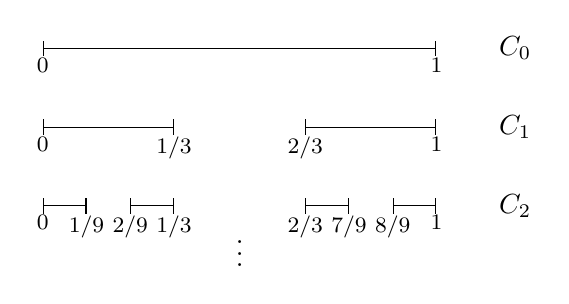
\begin{tikzpicture}
\draw[|-|] (0,0) node[below] {\footnotesize{\(0\)}} -- (5,0) node[below] {\footnotesize{\(1\)}};
\draw[|-|] (0,-1) node[below] {\footnotesize{\(0\)}} -- (\fpeval{5/3},-1) node[below] {\footnotesize{\(1/3\)}};
\draw[|-|] (\fpeval{10/3},-1) node[below] {\footnotesize{\(2/3\)}}-- (5,-1) node[below] {\footnotesize{\(1\)}};
\draw[|-|] (0,-2) node[below] {\footnotesize{\(0\)}} -- (\fpeval{5/9},-2) node[below] {\footnotesize{\(1/9\)}};
\draw[|-|] (\fpeval{2*5/9},-2) node[below] {\footnotesize{\(2/9\)}}-- (\fpeval{5/3},-2) node[below] {\footnotesize{\(1/3\)}};
\draw[|-|] (\fpeval{2*5/3},-2) node[below] {\footnotesize{\(2/3\)}} -- (\fpeval{7*5/9},-2) node[below] {\footnotesize{\(7/9\)}};
\draw[|-|] (\fpeval{8*5/9},-2) node[below] {\footnotesize{\(8/9\)}} -- (5,-2) node[below] {\footnotesize{\(1\)}};
\node[] () at (6,0) {\(C_0\)};
\node[] () at (6,-1) {\(C_1\)};
\node[] () at (6,-2) {\(C_2\)};
\node[] () at (2.5,-2.5) {\(\vdots\)};
\end{tikzpicture}
\end{center}

\begin{note}
It can be shown that \(\mathcal{C}=\{x\in[0,1]:x=\sum_{i=1}^{\infty}a_i3^{-i},
a_i\in\{0,2\}~\forall i\in\N\}\). The latter set contains all numbers in
\([0,1]\) whose base-3 expansion only has \(0\) or \(2\) as its digits.
The rough idea is that, the digits \(0\) or \(2\) correspond to the ``pieces''
remained in the picture above (in each step we are removing the ``middle
pieces'', corresponding to the digit \(1\)).
\end{note}

\begin{pf}
\begin{itemize}
\item \underline{\(\mathcal{C}\) is uncountable}: Assume to the contrary that
\(\mathcal{C}\) is countable and can be expressed as
\(\mathcal{C}=\{c_i:i\in\N\}\). List the \(c_i\)'s in the following way:
\begin{itemize}
\item \(c_1=0.\vc{0}00\cdots\)
\item \(c_2=0.0\orc{2}0\cdots\)
\item \(c_3=0.02\mgc{2}\cdots\)
\item \(\vdots\)
\end{itemize}
(the values here are for illustration only). By changing \(0\to 2\) and \(2\to
0\) in the each of the digits in the ``diagonal'' above, we can obtain
\(c=0.\vc{2}\orc{0}\mgc{0}\cdots\) (this value is for the example above), which
is guaranteed to be \emph{different} from every \(c_i\) in the list by
construction, meaning that \(c\notin\mathcal{C}\). However, we can certainly
write \(c=\sum_{i=1}^{\infty}a_i3^{-i}\) where \(a_i\in\{0,2\}\) for all
\(i\in\N\), contradiction.
\item \underline{\(\mathcal{C}\) is a Lebesgue null set}: Note that for every
\(i\in\N\), the set \(\mathcal{C}_i\) is obtained by removing \(2^{i-1}\)
intervals of length \(3^{-i}\) each from \(C_{i-1}\). Therefore, the length of
all the removed intervals is
\[
\lambda([0,1]\setminus\mathcal{C})=\sum_{i=1}^{\infty}2^{i-1}3^{-i}
=\frac{1}{2}\sum_{i=1}^{\infty}(2/3)^{i}
=\frac{1}{2}\left(\frac{1}{1-2/3}-1\right)
=1.
\]
Then, since \(1=\lambda([0,1])=\lambda(([0,1]\setminus \mathcal{C})\uplus\mathcal{C})
\overset{\text{(finite additivity)}}{=}\lambda([0,1]\setminus
\mathcal{C})+\lambda(\mathcal{C})=1+\lambda(\mathcal{C})\),
we have \(\lambda(\mathcal{C})=0\).
\end{itemize}
\end{pf}
\item[] \textbf{Lebesgue null sets in \(\R^d\)}
\item A line in \(\R^2\) is a Lebesgue null set.

\begin{pf}
WLOG, consider the line \(y=0\), i.e., \(\{(x,y)\in\R^2:y=0\}\), in
\(\R^2\).\footnote{Note that every line in \(\R^2\) can be obtained from this
line by translations, rotations, and reflections. As mentioned before, these
actions would not change the Lebesgue measure.} Write \(\Q=\{q_i:i\in\N\}\) and
fix any \(\varepsilon>0\). Let
\(A_i=(q_i-\varepsilon/2,q_i+\varepsilon/2]\times (-1/2^{i+1},1/2^{i+1}]\) for
every \(i\in\N\). Then we have \(\{(x,y)\in\R^2:y=0\}\subseteq
\bigcup_{i=1}^{\infty}A_i\), and thus
\[
0\le\lambda(\{(x,y)\in\R^2:y=0\})\le\lambda\left(\bigcup_{i=1}^{\infty}A_i\right)
\le\sum_{i=1}^{\infty}\mu(A_i)
=\sum_{i=1}^{\infty}\varepsilon\cdot 2^{-i}=\varepsilon.
\]
As this holds for every \(\varepsilon>0\), we conclude that
\(\lambda(\{(x,y)\in\R^2:y=0\})=0\).
\end{pf}

\begin{note}
Using a similar argument, we can show that any \(\R^k\) with \(k<d\) or its
subset is a Lebesgue null set in \(\R^d\), e.g., planes are Lebesgue null sets
in \(\R^3\).
\end{note}
\end{itemize}
\end{enumerate}
\subsection{Probability Measures}
\label{subsect:prob-meas}
\begin{enumerate}
\item \textbf{Terminologies.} Let \((\Omega,\mathcal{F})\) be a measurable
space. A \defn{probability measure} \(\pr\) on \(\mathcal{F}\) (or
\((\Omega,\mathcal{F})\)) is a function such that:
\begin{enumerate}[label={(\arabic*)}]
\item \emph{(nonnegativity)} \(\pr\) is a function from \(\mathcal{F}\) to \([0,\infty]\).
\item \emph{(unitarity)} \(\prob{\Omega}=1\).
\item \emph{(\(\sigma\)-additivity)} \(A_1,A_2,\dotsc\in\mathcal{F}\text{
pairwise disjoint}\implies
\prob{\biguplus_{i=1}^{\infty}A_i}=\sum_{i=1}^{\infty}\prob{A_i}\).
\end{enumerate}
The triple \((\Omega,\mathcal{F},\pr)\) is called a \defn{probability space},
\(\Omega\) is called a \defn{sample space}, and each outcome
\(\omega\in\Omega\) is called a \defn{sample point}. If \(\Omega\) is countable
(finite resp.), then \((\Omega,\mathcal{F},\pr)\) is said to be \defn{discrete}
(\defn{finite} resp.).  Every \(A\in\mathcal{F}\) is called an \defn{event}.

\item\label{it:prob-meas-prop} \textbf{Properties of probability measure.}
\begin{enumerate}
\item \emph{(probability measure is a measure)} We have
\(\prob{\varnothing}=0\), so the probability measure \(\pr\) can be identified
as a measure.

\begin{pf}
Let \(A_1=\Omega\) and \(A_i=\varnothing\) for every \(i=2,3,\dotsc\). Then we
have \(\Omega=\biguplus_{i=1}^{\infty}A_i\), thus
\[
1=\prob{\Omega}=\prob{\biguplus_{i=1}^{\infty}A_i}
=\sum_{i=1}^{\infty}\prob{A_i}
=\prob{\Omega}+\sum_{i=2}^{\infty}\prob{\varnothing},
\]
which implies that \(\sum_{i=2}^{\infty}\prob{\varnothing}=0\), forcing that
\(\prob{\varnothing}=0\).
\end{pf}
\item \emph{(numerous properties of measure)} Since \(\pr\) is a finite
measure, all properties in \labelcref{it:meas-prop} hold.
\end{enumerate}
\item \textbf{Examples of probability measures.}
\begin{enumerate}
\item\label{it:comb-prob} \emph{(combinatorial probability)} Let \(\Omega\) be
a finite sample space with \(\mathcal{F}=\mathcal{P}(\Omega)\).  Then we can
define \(\prob{A}:=|A|/|\Omega|\) for all \(A\in\mathcal{F}\), which is indeed
a probability measure on \(\mathcal{F}\).

\begin{pf}
\begin{enumerate}[label={(\arabic*)}]
\item Since \(0\le |A|\le |\Omega|\), we have \(0\le\prob{A}\le 1\) for all
\(A\in\mathcal{F}\), so \(\pr\) can be considered to be a function from
\(\mathcal{F}\) to \([0,1]\).
\item We have \(\prob{\Omega}=|\Omega|/|\Omega|=1\).
\item Fix any pairwise disjoint \(A_1,A_2,\dotsc\in\mathcal{F}\). Noting that
\(\left|\biguplus_{i=1}^{\infty}A_i\right|=\sum_{i=1}^{\infty}|A_i|\), we have
\[
\prob{\biguplus_{i=1}^{\infty}A_i}
=\frac{\left|\biguplus_{i=1}^{\infty}A_i\right|}{|\Omega|}
=\sum_{i=1}^{\infty}\frac{|A_i|}{|\Omega|}
=\sum_{i=1}^{\infty}\prob{A_i}.
\]
\end{enumerate}
\end{pf}
\item \emph{(defined via mass function)} Let \(\Omega\) be a countable sample
space with \(\mathcal{F}=\mathcal{P}(\Omega)\). Then any \defn{mass function}
\(f:\Omega\to[0,1]\) with \(\sum_{\omega\in\Omega}^{}f(\omega)=1\) induces a
\defn{discrete probability measure} \(\pr\) on \(\mathcal{F}\) by
\(\prob{A}=\sum_{\omega\in A}^{}f(\omega)\) for all \(A\in\mathcal{F}\).

\begin{remark}
\item Conversely, if \(\pr\) is a probability measure on \(\mathcal{F}\), then
\(f(\omega):=\prob{\{\omega\}}\) is the corresponding pmf that induces \(\pr\).
\item The argument for showing such \(\pr\) is indeed a probability measure is
analogous to that in \labelcref{it:meas-sum-fn}.
\end{remark}
\item \emph{(geometric probability space)} Let the sample space \(\Omega\) be a
subset of \(\R^d\) with \(\lambda(\Omega)<\infty\) and
\(\mathcal{F}=\bar{\mathcal{B}}(\Omega)\). Define
\(\prob{A}=\lambda(A)/\lambda(\Omega)\) for all \(A\in\mathcal{F}\)
\emph{(relative volume)}. Then \(\pr\) is a probability measure on
\(\mathcal{F}\) (which can be proved using a similar argument as in
\labelcref{it:comb-prob}). Here, \((\Omega,\mathcal{F},\pr)\) is called
\defn{geometric probability space}.
\end{enumerate}
\item \textbf{Characterization of probability measures on \(\R^d\).} In the
case where \(\Omega=\R^d\), there is a characterization of the probability
measure through the \emph{distribution function}. It is indeed the one you have
learnt in your first course in probability, but here we will define it in a way
that does not involve the notion of ``random variable'' (as we have not yet
defined it formally!).

A \defn{(multivariate/joint) distribution function} is a function
\(F:\R^d\to[0,1]\) such that:
\begin{enumerate}[label={(\arabic*)}]
\item \(\lim_{x_j\to\infty}F(\vect{x})=0\) for all \(j=1,\dotsc,d\) \emph{(groundedness)}
and \(\lim_{\vect{x}\to\vect{\infty}}F(\vect{x})=1\) \emph{(normalization)}.
\item \(F\) is \(d\)-increasing.
\item \(F\) is right-continuous.
\end{enumerate}
The following result then tells us how distribution function characterizes
probability measures on \(\R^d\).
\begin{theorem}
\label{thm:dist-fn-char-prob-meas-rd}
Let \(\Omega=\R^d\). Then:
\begin{enumerate}
\item \emph{\(\pr\) induces \(F\):} If \(\pr\) is a probability measure on
\(\bar{\mathcal{B}}(\R^d)\), then
\orc{\(F(\vect{x}):=\prob{(\vect{-\infty},\vect{x}]}\)} is a distribution function.
Also, we have \vc{\(\lambda_F=\pr\)} for this \(F\).
\item \emph{\(F\) induces \(\pr\):} If \(F\) is a distribution function, then
\vc{\(\pr:=\lambda_{F}\)} is a probability measure on \(\bar{\mathcal{B}}(\R^d)\).
Also, we have \orc{\(\prob{(\vect{-\infty},\vect{x}]}=F(\vect{x})\)} for all
\(\vect{x}\in\R^d\) for this \(\pr\).
\end{enumerate}
\end{theorem}
\begin{center}
\begin{tikzpicture}
\node[scale=2] () at (0,0) {\(\pr\)};
\node[scale=2] () at (5,0) {\(F\)};
\node[scale=2] () at (10,0) {\(\pr\)};
\draw[-Latex] (0.5,0) --node[midway,above]{\orc{\(F(\vect{x}):=\prob{(\vect{-\infty},\vect{x}]}\)}} (4.5,0);
\node[] () at (5,-0.5) {(\vc{\(\lambda_F=\pr\)})};
\draw[-Latex] (5.5,0) --node[midway,above]{\vc{\(\pr:=\lambda_{F}\)}} (9.5,0);
\end{tikzpicture}
\begin{tikzpicture}
\node[scale=2] () at (0,0) {\(F\)};
\node[scale=2] () at (5,0) {\(\pr\)};
\node[scale=2] () at (10,0) {\(F\)};
\draw[-Latex] (0.5,0) --node[midway,above]{\vc{\(\pr:=\lambda_{F}\)}} (4.5,0);
\node[] () at (5,-0.5) {(\orc{\(\prob{(\vect{-\infty},\vect{x}]}=F(\vect{x})\)})};
\draw[-Latex] (5.5,0) --node[midway,above]{\orc{\(F(\vect{x}):=\prob{(\vect{-\infty},\vect{x}]}\)}} (9.5,0);
\end{tikzpicture}
\end{center}
\begin{remark}
\item As the picture above illustrates, the two ways (mappings) of getting from
\(\pr\) to \(F\) and \(F\) to \(\pr\) are inverse to each other (applying one
after another would yield an identity mapping), thus forming a one-to-one
correspondence between the probability measures and distribution functions.
\item The distribution function
\(F(\vect{x}):=\prob{(\vect{-\infty},\vect{x}]}\) is called the
\defn{distribution function of \(\pr\) (or \(\lambda_{F}\))}.
\item For every probability measure \(\pr\) on \(\bar{\mathcal{B}}(\R^d)\) with
distribution function \(F\), we have
\(\prob{(\vect{a},\vect{b]}}=\lambda_{F}(\vect{a},\vect{b}]=\Delta_{(\vect{a},\vect{b}]}F\).
This gives rise to another interpretation of the \(F\)-volume
\(\Delta_{(\vect{a},\vect{b}]}F\), namely that it is the probability of
\((\vect{a},\vect{b}]\) under the distribution function \(F\).
\end{remark}

\begin{pf}
\begin{enumerate}
\item We first show that \(F(\vect{x}):=\prob{(\vect{-\infty},\vect{x}]}\) is a
distribution function.
\begin{enumerate}[label={(\arabic*)}]
\item Note that \(\lim_{x_j\to\infty}F(\vect{x})
=\lim_{n\to\infty}F(\vect{x}_{j\leftarrow -n}
=\lim_{n\to\infty}\prob{(\vect{-\infty},\vect{x}_{j\leftarrow -n}}
\) for all \(j=1,\dotsc,d\), and
\(F(\vect{\infty})=\lim_{n\to\infty}\prob{(\vect{-\infty},{}_{d}n]}
\overset{\text{(continuity from below)}}{=}\prob{\bigcup_{n=1}^{\infty}(\vect{-\infty},{}_{d}n]}
=\prob{\R^d}=\prob{\Omega}=1\).
\item Note first that
\begin{align*}
\Delta_{(a_1,b_1]}F&=F(b_1,x_2,\dotsc,x_d)-F(a_1,x_2,\dotsc,x_d) \\
&=\prob{(\vect{-\infty},(b_1,x_2,\dotsc,x_d)]}
-\prob{(\vect{-\infty},(a_1,x_2,\dotsc,x_d)]} \\
\overset{\text{(subtractivity)}}&{=}
\prob{(\vect{-\infty},(b_1,x_2,\dotsc,x_d)]
\setminus(\vect{-\infty},(a_1,x_2,\dotsc,x_d)]} \\
&=\prob{\left(\begin{bmatrix}a_1\\ \vect{-\infty}\end{bmatrix},
\begin{bmatrix}b_1\\ \vect{x}_{\{1\}^{c}}\end{bmatrix}\right]}.
\end{align*}
Hence, for all \(\vect{a}\le\vect{b}\), applying an argument similar to above
repetitively gives
\begin{align*}
\Delta_{(\vect{a},\vect{b}]}F&=\Delta_{(a_d,b_d]}\cdots\Delta_{(a_2,b_2]}\Delta_{(a_1,b_1]}F \\
&=\Delta_{(a_d,b_d]}\cdots\Delta_{(a_2,b_2]}
\prob{\left(\begin{bmatrix}a_1\\ \vect{-\infty}\end{bmatrix},
\begin{bmatrix}b_1\\ \vect{x}_{\{1\}^{c}}\end{bmatrix}\right]} \\
&=\cdots=\prob{(\vect{a},\vect{b}]}\ge 0,
\end{align*}
establishing the \(d\)-increasingness.
\item For all \(\vect{x}\le\vect{y}\), we have
\(F(\vect{x})=\prob{(\vect{-\infty},\vect{x}]}
\overset{\text{(monotonicity)}}{\le}\prob{(\vect{-\infty},\vect{y}]}=F(\vect{y})\).
Thus,
\begin{align*}
\lim_{\vect{h}\to\vect{0}^{+}}F(\vect{x}+\vect{h})
&=\lim_{\vect{n}\to\vect{\infty}}F(\vect{x}+\vect{1/n})
\le\lim_{\min_{j}\{n_j\}\to \infty}
F\left(\vect{x}+{}_{d}\left(\frac{1}{\min_{j}\{n_j\}}\right)\right) \\
\overset{\text{(relabel \(m=\min_{j}\{n_j\}\))}}&{=}
\lim_{m\to\infty}F(\vect{x}+{}_{d}(1/m))
=\lim_{m\to\infty}\prob{(\vect{-\infty},\vect{x}+{}_{d}(1/m)]} \\
\overset{\text{(continuity from above)}}&{=}
\prob{\bigcap_{m=1}^{\infty}(\vect{-\infty},\vect{x}+{}_{d}(1/m)]}
=\prob{(\vect{-\infty},\vect{x}]}
=F(\vect{x}),
\end{align*}
for all \(\vect{x}\in\R^d\).  Changing \(\min_{j}\to\max_{j}\) above gives
\(\lim_{\vect{h}\to\vect{0}^{+}}F(\vect{x}+\vect{h})\ge F(\vect{x})\) for all
\(\vect{x}\in\R^d\). Hence, together with the inequality above, we get
\(\lim_{\vect{h}\to\vect{0}^{+}}F(\vect{x}+\vect{h})= F(\vect{x})\) for all
\(\vect{x}\in\R^d\).
\end{enumerate}
Next, we show that \(\lambda_{F}=\pr\). Here it suffices to show this equality
on \(\mathcal{B}(\R^d)\) (rather than \(\bar{\mathcal{B}}(\R^d)\)) as
completion of measure is done uniquely by \Cref{thm:complete-meas}. Also, by
\Cref{prp:meas-unique}, it suffices to show that \(\lambda_{F}=\pr\) on the
\(\pi\)-system \(\mathcal{A}=\{(\vect{-\infty},\vect{b}]:\vect{b}\in\R^d\}\)
since \(\sigma(\mathcal{A})=\mathcal{B}(\R^d)\) by
\Cref{prp:borel-rd-generators}.  This follows from the observation that
\[
\lambda_{F}((\vect{-\infty},\vect{b}])=\Delta_{(\vect{-\infty},\vect{b}]}F
\underset{\text{(\(F\) grounded)}}{\overset{\text{\labelcref{it:ground-lim}}}{=}}F(\vect{b})
=\prob{(\vect{-\infty},\vect{b}]}
\]
for all \(\vect{b}\in\R^d\).

\item By \Cref{thm:construct-borel-meas-rd}, we know there is a unique Borel
measure \(\lambda_{F}\) such that
\(\lambda_{F}(\vect{a},\vect{b}]=\Delta_{(\vect{a},\vect{b}]}F\) for all
\(\vect{a}\le\vect{b}\). We now show that \(\lambda_{F}\) is a probability
measure on \(\bar{\mathcal{B}}(\R^d)\).
\begin{enumerate}[label={(\arabic*)}]
\item The nonnegativity of \(\lambda_{F}\) follows from the fact that
\(\lambda_{F}\) is a measure.
\item Note that
\begin{align*}
\lambda_{F}(\R^d)\overset{\text{(continuity from below)}}&{=}
\lim_{n\to\infty}\lambda_{F}((-{}_{d}n,{}_{d}n])
=\lim_{n\to\infty}\Delta_{(-{}_{d}n,{}_{d}n]}F \\
&=\lim_{n\to\infty}\sum_{\vect{i}\in\{0,1\}^{d}}^{}
(-1)^{\sum_{j=1}^{d}i_j}F((-1)^{i_1}n,\dotsc,(-1)^{i_d}n) \\
&=\sum_{\vect{i}\in\{0,1\}^{d}}^{}(-1)^{\sum_{j=1}^{d}i_j}
\lim_{n\to\infty}F((-1)^{i_1}n,\dotsc,(-1)^{i_d}n).
\end{align*}
Since
\[
\lim_{n\to\infty}F((-1)^{i_1}n,\dotsc,(-1)^{i_d}n)
=\begin{cases}
0&\text{if \(i_j=1\) for some \(j\) by groundedness,} \\
F(\vect{\infty})=1&\text{if \(\vect{i}=\vect{0}\),} \\
\end{cases}
\]
we conclude that \(\lambda_{F}(\R^d)=1\).
\item The \(\sigma\)-additivity follows from the fact that \(\lambda_{F}\) is a measure.
\end{enumerate}
Next, the result \(\prob{(\vect{-\infty},\vect{x}]}=F(\vect{x})\) follows by
noting that
\begin{align*}
\prob{(\vect{-\infty},\vect{x}]}
&=\lambda_{F}((\vect{-\infty},\vect{x}])
\overset{\text{(continuity from below)}}{=}
\lim_{n\to\infty}\lambda_{F}((-{}_{d}n,\vect{x}]) \\
&=\lim_{n\to\infty}\Delta_{(-{}_{d}n,\vect{x}]}F
=\Delta_{(\vect{-\infty},\vect{x}]}F
\overset{\text{\labelcref{it:ground-lim}}}{=}F(\vect{x})
\end{align*}
for all \(\vect{x}\in\R^d\).
\end{enumerate}
\end{pf}
\item \textbf{Discrete, absolutely continuous, and continuous singular
distribution functions.} In your first probability course, you should have
learnt the concepts of \emph{discrete} and \emph{(absolutely) continuous}
random variables. Here, we will explore similar ideas for distribution
functions, \emph{without} involving the notions of random variables. Also, we
will introduce the concept of \emph{continuous singular distribution function}
which, together with the discrete and absolutely continuous distribution
functions, can represent \emph{any} distribution function through a mixture.

Let \(F\) be a distribution function. The \defn{support} of \(F\) is given by
\(\supp{F}:= \{\vect{x}\in\R^d:\Delta_{(\vect{x}-\vect{h},\vect{x}]}F>0\text{
for all }\vect{h}>\vect{0}\}\), which is the set of all inputs that get
positive probability assigned in the ``neighbouring'' region (recall that we
can view \(\Delta_{(\vect{x}-\vect{h},\vect{x}]}F\) as the probability
\(\prob{(\vect{x}-\vect{h},\vect{x}]}\)). \begin{note}
Here we consider the condition ``\(\Delta_{(\vect{x}-\vect{h},\vect{x}]}F>0\)
for all \(\vect{h}>\vect{0}\)'', rather than the more
natural``\(F(\vect{x})>0\)'', mainly for mathematical convenience.
This can exclude some ``edge cases'' in the support.
\end{note}

While the domain of the distribution function \(F\) is \(\R^d\), often we are
only interested in its behaviour in the support \(\supp{F}\); the values taken
outside \(\supp{F}\) should always be \(1\) in the ``upper-right'' part
(corresponding the \emph{normalization} condition), and \(0\) in the other
parts (corresponding to the \emph{groundedness} condition). Functions defined
on subsets of \(\R^d\) may then be treated as ``distribution function'' with
the understanding that they are to be extended in this way to make their
domains being \(\R^d\).

Now, we are ready to define the three kinds of distribution functions:
\begin{itemize}
\item A distribution function \(F\) is \defn{discrete} if \(\supp{F}\) is
countable, and its \defn{mass function} is given by
\(f(\vect{x})=\prob{\{\vect{x}\}}
=\Delta_{(\vect{x}-,\vect{x}]}F
:=\lim_{\vect{a}\to \vect{x}^{-}}\Delta_{(\vect{a},\vect{x}]}F\).

\begin{note}
We can show \(\prob{\{\vect{x}\}} =\Delta_{(\vect{x}-,\vect{x}]}F\) by:
\begin{align*}
\prob{\{\vect{x}\}}&=\prob{\bigcap_{n=1}^{\infty}(\vect{x}-{}_{d}(1/n),\vect{x}]}
\overset{\text{(continuity from above)}}{=}
\lim_{n\to\infty}\prob{\left(\vect{x}-{}_{d}(1/n),\vect{x}\right]} \\
&=\lim_{n\to\infty}\lambda_{F}\left(\left(\vect{x}-{}_{d}(1/n),\vect{x}\right]\right)
=\lim_{n\to\infty}\Delta_{\left(\vect{x}-{}_{d}(1/n),\vect{x}\right]}F
=\Delta_{(\vect{x}-,\vect{x}]}F.
\end{align*}
\end{note}
\item A distribution function \(F\) is \defn{absolutely continuous} if we can write
\[
F(\vect{x})=\int_{\vect{-\infty}}^{\vect{x}}f(\vect{t})\odif{\vect{t}}
\]
for all \(\vect{x}\in\R^d\), where \(f:\R^d\to[0,\infty)\) is an
\emph{integrable} function with
\(\int_{\vect{-\infty}}^{\vect{\infty}}f(\vect{t})\odif{\vect{t}}=1\) (the
concept of integrability will be discussed in
\Cref{sect:integration-expectation}). Such \(f\) is called the \defn{density
function} of \(F\). If \(\pdv{}{\vect{x}}F(\vect{x})\) exists almost everywhere
(with respect to the Lebesgue measure), then such \(f\) can be obtained by
\(f(\vect{x})=\pdv{}{\vect{x}}F(\vect{x})\) almost everywhere (and the values
taken by \(f\) outside the ``almost everywhere'' case would not affect the integral).
\item A distribution function \(F\) is \defn{continuous singular} if \(F\) is a
continuous function with \(\pdv{}{\vect{x}}F(\vect{x})=0\) almost everywhere.
\end{itemize}
\item\label{it:dist-fn-fmla} \textbf{Formulas for distribution functions.}
\begin{enumerate}
\item \emph{(absolutely continuous distribution function)} If \(F\) is
absolutely continuous with density \(f\), then
\(\prob{(\vect{a},\vect{b}]}=\int_{(\vect{a},\vect{b}]}^{}f(\vect{t})\odif{\vect{t}}\)
(this should be somewhat familiar to you already \faIcon[regular]{grin-wink}).

\begin{pf}
We have
\begin{align*}
\prob{(\vect{a},\vect{b}]}
&=\Delta_{(\vect{a},\vect{b}]}F
=\Delta_{(a_1,b_1]}\cdots\Delta_{(a_d,b_d]}
\int_{-\infty}^{x_d}\dotsb\int_{-\infty}^{x_1}f(t_1,\dotsc,t_d)\odif{t_1}\cdots\odif{t_d} \\
&=\int_{a_d}^{b_d}\dotsb\int_{a_1}^{b_1}f(t_1,\dotsc,t_d)\odif{t_1}\cdots\odif{t_d}
=\int_{(\vect{a},\vect{b}]}^{}f(\vect{t})\odif{\vect{t}}.
\end{align*}
\end{pf}
\item \emph{(mixture representation)} Every distribution function \(F\) admits
the following mixture representation
\[
F(\vect{x})=p_{\mathrm{d}}F_{\mathrm{d}}(\vect{x})+
p_{\mathrm{ac}}F_{\mathrm{ac}}(\vect{x})+
p_{\mathrm{cs}}F_{\mathrm{cs}}(\vect{x})
\]
where \(p_{\mathrm{d}},p_{\mathrm{ac}},p_{\mathrm{cs}}\ge 0\) with
\(p_{\mathrm{d}}+p_{\mathrm{ac}}+p_{\mathrm{cs}}=1\), and
\(F_{\mathrm{d}},F_{\mathrm{ac}},F_{\mathrm{cs}}\) are discrete, absolutely
continuous, and continuous singular distribution functions respectively.

\begin{pf}
Omitted.
\end{pf}
\item \emph{(margins of distribution functions)} For every \(J\subseteq
\{1,\dotsc,d\}\), the \defn{\(J\)-margin} of \(F\) is given by
\(F_J(\vect{x}_J):=\lim_{\vect{x}_{J^c}\to\vect{\infty}}F(\vect{x})\).  In the
special case where \(J=\{j\}\) for some \(j=1,\dotsc,d\), it is further called
the \defn{\(j\)th margin of \(F\)}, which is
\(F_j(x_j)=\lim_{\vect{x}_{j^c}\to\vect{\infty}}F(\vect{x})\). Applying a similar
idea to events, for all \(A=\prod_{j=1}^{d}A_j\in\bar{\mathcal{B}}(\R^d)\), we
write \(\prob{A_J}=\prob{\prod_{j\in J}A_j}:=\prob{\prod_{j=1}^{d}B_j}\)
where \(B_j=A_j\) for all \(j\in J\) and \(B_j=\Omega\) for all \(j\notin J\).

Then, we have:
\begin{enumerate}
\item \(F_J(\vect{x}_J)=\prob{(\vect{-\infty},\vect{x}_{J}]}\) for every
\(J\subseteq \{1,\dotsc,d\}\).
\item \(F_j(x_j)=\prob{(-\infty,x_{j}]}\) for every \(j=1,\dotsc,d\).
\item \(\prob{(a_j,b_j]}=F_{j}(b_j)-F_{j}(a_j)\) for every \(j=1,\dotsc,d\).
\end{enumerate}
Here \(F\) is supposed to be the distribution function of \(\pr\).

\begin{pf}
\begin{enumerate}
\item We have \(F_{J}(\vect{x}_J)=\lim_{\vect{x}_{J^c}\to\vect{\infty}}F(\vect{x})
\overset{\text{(\Cref{thm:dist-fn-char-prob-meas-rd})}}{=}\lim_{\vect{x}_{J^c}\to\vect{\infty}}\prob{(\vect{-\infty},\vect{x}]}
\overset{\text{(continuity from below)}}{=}
\prob{(\vect{-\infty},\vect{x}_{J}]}\).
\item Take \(J=\{j\}\) from above.
\item We have \(\prob{(a_j,b_j]}=\prob{(-\infty,b_j]\setminus (-\infty,a_j]}
=\prob{(-\infty,b_j]}-\prob{(-\infty,a_j]}=F_j(b_j)-F_j(a_j)\).
\end{enumerate}
\end{pf}
\end{enumerate}
\item\label{it:abs-cts-df-cts} \textbf{Continuity of absolutely continuous distribution functions.}
As one would expect, absolutely \underline{continuous} distribution functions
are indeed continuous. We need the following lemma to prove this property.
\begin{lemma}[Lipschitz inequality]
\label{lma:lipschitz-ineq}
If \(F\) is \(d\)-increasing and grounded, then
\[
|F(\vect{b})-F(\vect{a})|\le\sum_{j=1}^{d}|F_j(b_j)-F_j(a_j)|
\]
for all \(\vect{a},\vect{b}\in\R^d\).
\end{lemma}
\begin{pf}
Since \(F(\vect{b})-F(\vect{a})=\sum_{j=1}^{d}[F(b_1,\dotsc,b_{j-1},b_j,a_{j+1},\dotsc,a_d)
-F(b_1,\dotsc,b_{j-1},a_j,a_{j+1},\dotsc,a_d)]\), by triangle inequality we have
\[
|F(\vect{b})-F(\vect{a})|\le\sum_{j=1}^{d}|F(b_1,\dotsc,b_{j-1},b_j,a_{j+1},\dotsc,a_d)
-F(b_1,\dotsc,b_{j-1},a_j,a_{j+1},\dotsc,a_d)|.
\]
Fix any \(j\in\{1,\dotsc,d\}\).  WLOG, suppose \(a_j\le b_j\). Then for the
\(j\)th summand we have
\begin{align*}
&|F(b_1,\dotsc,b_{j-1},b_j,a_{j+1},\dotsc,a_d)
-F(b_1,\dotsc,b_{j-1},a_j,a_{j+1},\dotsc,a_d)| \\
\overset{\text{\labelcref{it:f-vol-nonneg}}}&{=}
F(\vc{b_1},\dotsc,b_{j-1},\vc{b_j},a_{j+1},\dotsc,a_d)
-F(\vc{b_1},\dotsc,b_{j-1},\vc{a_j},a_{j+1},\dotsc,a_d) \\
\overset{\text{\labelcref{it:f-vol-nonneg}}}&{\le}
F(\vc{\infty},\orc{b_{2}},\dotsc,b_{j-1},\vc{b_j},a_{j+1},\dotsc,a_d)
-F(\vc{\infty},\orc{b_{2}},\dotsc,b_{j-1},\vc{a_j},a_{j+1},\dotsc,a_d) \\
\overset{\text{\labelcref{it:f-vol-nonneg}}}&{\le}
F(\infty,\orc{\infty},\dotsc,b_{j-1},\vc{b_j},a_{j+1},\dotsc,a_d)
-F(\infty,\orc{\infty},\dotsc,b_{j-1},\vc{a_j},a_{j+1},\dotsc,a_d) \\
\overset{\text{\labelcref{it:f-vol-nonneg}}}
&{\le\cdots\le} F_j(b_j)-F_j(a_j) \\
\overset{\text{\labelcref{it:f-vol-nonneg}}}&{=}
|F_j(b_j)-F_j(a_j)|.
\end{align*}
Hence the result follows.
\end{pf}

With \Cref{lma:lipschitz-ineq}, we can obtain a sufficient condition for the
continuity of distribution function.
\begin{proposition}
\label{prp:marg-cts-df-cts}
If the margins \(F_1,\dotsc,F_d\) of \(F\) are all continuous, then so is \(F\).
\end{proposition}
\begin{note}
The condition is particularly satisfied by absolutely continuous distribution
functions, whose margins are given by
\(F_j(x_j)=\prob{(-\infty,x_j]}=\int_{-\infty}^{x_j}f(t)\odif{t}\) for all
\(j=1,\dotsc,d\), which are all continuous by the fundamental theorem of
calculus.
\end{note}

\begin{pf}
Assume the margins \(F_1,\dotsc,F_d\) of \(F\) are all continuous. Then consider:
\[
\lim_{\vect{h}\to \vect{0}}|F(\vect{x})-F(\vect{x}-\vect{h})|
\overset{\text{(\Cref{lma:lipschitz-ineq})}}{\le}
\lim_{\vect{h}\to \vect{0}}\sum_{j=1}^{d}|F_j(x_j)-F_j(x_j-h_j)|
\overset{\text{(\(F_j\)'s continuous)}}{=}0,
\]
which implies that \(\lim_{\vect{h}\to
\vect{0}}F(\vect{x}-\vect{h})=F(\vect{x})\), and hence \(F\) is continuous.
\end{pf}
\item\label{it:cts-df-not-abs-cts} \textbf{An example of continuous distribution function that is not
absolutely continuous.}
While we know from \labelcref{it:abs-cts-df-cts} that absolutely continuous
distribution functions are always continuous, the converse does not hold. A
standard counterexample is the \emph{Cantor distribution function}, a.k.a.\ the
\emph{devil's staircase}.

Recall the Cantor set \(\mathcal{C}=\{x\in[0,1]:x=\sum_{i=1}^{\infty}a_i3^{-i},
a_i\in\{0,2\}~\forall i\in\N\}\). Then the \defn{Cantor distribution function} \(F\)
is defined by
\begin{itemize}
\item \(F(x):=\sum_{i=1}^{\infty}\frac{a_i}{2}2^{-i}\) for every
\(x=\sum_{i=1}^{\infty}a_i3^{-i}\in\mathcal{C}\), which gives the base-2
expansions of all the numbers in \([0,1]\) (hence \(F(\mathcal{C})=[0,1]\)), and
\item \(F(x)=\sup_{y\le x, y\in\mathcal{C}}F(y)\) for all
\(x\in\mathcal{C}^c\).
\end{itemize}
The Cantor distribution function \(F\) can be shown to
be continuous, but \(F\) is \emph{not} absolutely continuous, since if a
density \(f\) existed, then we would have \(f(t)=0\) for all
\(t\in\mathcal{C}^c\) and so \(\int_{[0,1]}^{}f(t)\odif{t}=\int_{\mathcal{C}}^{}f(t)\odif{t}
+\int_{\mathcal{C}^c}^{}f(t)\odif{t}=0+0=0\ne 1\), as the integral over a
Lebesgue null set is always zero (see \Cref{sect:integration-expectation}).
\begin{note}
The Cantor distribution function is also an example of \emph{continuous
singular} distribution function.
\end{note}
\item \textbf{Quantile functions.} Apart from distribution function, the
probability measure can also be characterized by a \emph{quantile function},
whose graph is obtained by reflecting the graph of distribution function along
the line \(y=x\), with flat parts and jumps interchanged:
\begin{center}
\begin{tikzpicture}[scale=0.9]
\begin{axis}[domain=0:5, axis lines=middle, samples=100,
ymax=5.5, ytick={5}, yticklabels={1},
xtick=\empty, ylabel={\(y\)},xlabel={\(x\)},
xlabel style={anchor=west},
ylabel style={anchor=south},
]
\addplot[blue, domain=0:2]{x^(1/2)};
\addplot[blue, domain=3:5]{2.5+x/2};
\draw[blue, fill] (2,4) circle [radius=0.8mm];
\addplot[blue, domain=2:3]{4};
\node[blue] () at (2.5,1) {\(y=F(x)\)};
\draw[dashed, blue] (2,\fpeval{2^(1/2)}) -- (2,4);
\addplot[magenta, dotted]{x};
\node[magenta] () at (3,3) {\(y=x\)};
\end{axis}
\end{tikzpicture}
\begin{tikzpicture}[scale=0.9]
\begin{axis}[domain=0:5, axis lines=middle, samples=100, xmax=5.5,
ymax=5.5, xtick={5}, xticklabels={1}, xticklabel style={yshift=0.6cm},
ytick=\empty, ylabel={\(x\)},xlabel={\(y\)},
xlabel style={anchor=west},
ylabel style={anchor=south},
]
\addplot[ForestGreen, domain=0:\fpeval{2^(1/2)}]{x^2};
\addplot[ForestGreen, domain=4:5]{-5+2*x};
\draw[ForestGreen, fill] (4,2) circle [radius=0.8mm];
\addplot[ForestGreen, domain=\fpeval{2^(1/2)}:4]{2};
\node[ForestGreen] () at (1,2.5) {\(x=F^{-1}(y)\)};
\draw[dashed, ForestGreen] (4,2) -- (4,3);
\addplot[magenta, dotted]{x};
\node[magenta] () at (3,3) {\(y=x\)};
\end{axis}
\end{tikzpicture}
\end{center}
More formally, the notion of \emph{generalized inverse} is used in the
definition of quantile function. Let \(F:\R\to\R\) be an increasing function.
Then the \defn{generalized inverse} of \(F\) is a function \(F^{-1}:\R\to\eR\)
defined by
\[
F^{-1}(y):=\inf\{x\in\R:F(x)\ge y\}\quad\text{for all \(y\in\R\),}
\]
where we have \(\inf\varnothing:=\infty\) conventionally. If \(F\) is a
distribution function (with codomain being \([0,1]\) instead of \(\R\)), the
generalized inverse is defined in the same way except that its domain becomes
\([0,1]\). In such case, the generalized inverse \(F^{-1}:[0,1]\to\eR\) is
called the \defn{quantile function} of \(F\).

\item \label{it:gen-inv-prop} \textbf{Properties of generalized inverses.}
While the inverse function notation \(F^{-1}\) is used to denote generalized
inverse, there are indeed some subtle differences between the generalized
inverse and the ordinary inverse. Notably, the ordinary inverse only exists if
the underlying function is bijective, but the generalized inverse \emph{always}
exists, even if the underlying function has jumps and/or flat parts. It is thus
instructive to study some properties of generalized inverse. In the following,
we will just assume that \(F\) is increasing unless otherwise specified. Also,
we write \(F(-\infty):=\lim_{x\to -\infty}F(x)\) and \(F(\infty):=\lim_{x\to
\infty}F(x)\).
\begin{enumerate}
\item \emph{(behaviour of \(F^{-1}\))}
\begin{enumerate}
\item \emph{(increasing)} \(F^{-1}\) is increasing.
\item \emph{(left-continuous)} If \(-\infty<F^{-1}(y)<\infty\), then \(F^{-1}\)
is left-continuous at \(y\).
\end{enumerate}
\item \emph{(sufficient condition for coinciding with ordinary inverse)} If the
underlying function \(F\) is \emph{strictly} increasing and continuous, then
the generalized inverse \(F^{-1}\) coincides with the ordinary inverse of
\(F\) on \(\ran{F}\).
\item \emph{(behaviour of \(F^{-1}(F(\cdot))\))}
\begin{enumerate}
\item \emph{(``\(\leq\)'')} Generally, we have \(F^{-1}(F(x))\le x\).
\item \emph{(``\(=\)'')} If \(F\) is \emph{strictly} increasing, then we have \(F^{-1}(F(x))=x\).
\end{enumerate}
\item \emph{(behaviour of \(F(F^{-1}(\cdot))\))} Suppose that \(F\) is
right-continuous.
\begin{enumerate}
\item \emph{(``\(\ge\)'')} If \(F^{-1}(y)<\infty\), then \(F(F^{-1}(y))\ge y\).
\item \emph{(``\(=\)'')} Furthermore, if \(y\in\ran{F}\cup\{\inf\ran{F},\sup\ran{F}\}\), then \(F(F^{-1}(y))=y\).
\item \emph{(``\(>\)'')} If \(y<\inf\ran{F}\), then \(F(F^{-1}(y))>y\).
\item \emph{(``\(<\)'')} If \(y>\sup\ran{F}\), then \(F(F^{-1}(y))<y\).
\end{enumerate}
\item \emph{(inequalities about generalized inverse)}
\begin{enumerate}
\item \emph{(``applying'' \(F^{-1}\) preserves ``\(\ge\)'')} If \(F(x)\ge y\), then \(x\ge F^{-1}(y)\).
\item \emph{(``iff'' for ``\(\ge\)'' under right-continuity)} Suppose that
\(F\) is right-continuous. Then, \(F(x)\ge y\) iff \(x\ge F^{-1}(y)\).
\item \emph{(``applying'' \(F^{-1}\) turns ``\(<\)'' to ``\(\le\)'')} If \(F(x)<y\), then \(x\le F^{-1}(y)\).
\end{enumerate}
\item \emph{(relationship between continuity and strict increasingness)}
\begin{enumerate}
\item \(F\) is continuous iff \(F^{-1}\) is strictly increasing on \([\inf\ran{F},\sup\ran{F}]\).
\item \(F\) is strictly increasing iff \(F^{-1}\) is continuous on \(\ran{F}\).
\end{enumerate}
\end{enumerate}
\begin{pf}
Omitted; see \textcite{embrechts2013note}.
\end{pf}
\end{enumerate}
